\chapter{Discussion}\label{chp:discussion}

A comprehensive discussion on the findings will now be presented, first on the experiment and then on the model.

\section{Experiment}
% why do we prefer spark ignition
This project was started on the heels of \textcite{duplayArgonLaserPlasmaThruster2024a}, with the V1 test section using wire initiation. In this experiment, spark initiation was preferred to wire initiation for a few reasons. First, there would be no solid object blocking the beam path. This would allow the power meter to measure the energy that was not absorbed by the plasma. Second, replacing the target wire was a time-consuming process that was conducted every 1–3 shots, requiring the test section to be re-pressurized. Indeed, spark initiation enabled a much higher shot rate. Third, when conducting flowing experiments, the wire could be moved out of the focus by the flowing argon. Finally, the wire prevented the downstream propagation of the plasma by being physically in the way.

With V1, spark initiation was first attempted with two side by side electrodes that could fit into a single port, seen in \autoref{fig: V1 single plug electrodes}. However, the spark was created at a different height every time between the parallel electrodes.

\begin{figure}[!ht]
    \centering
    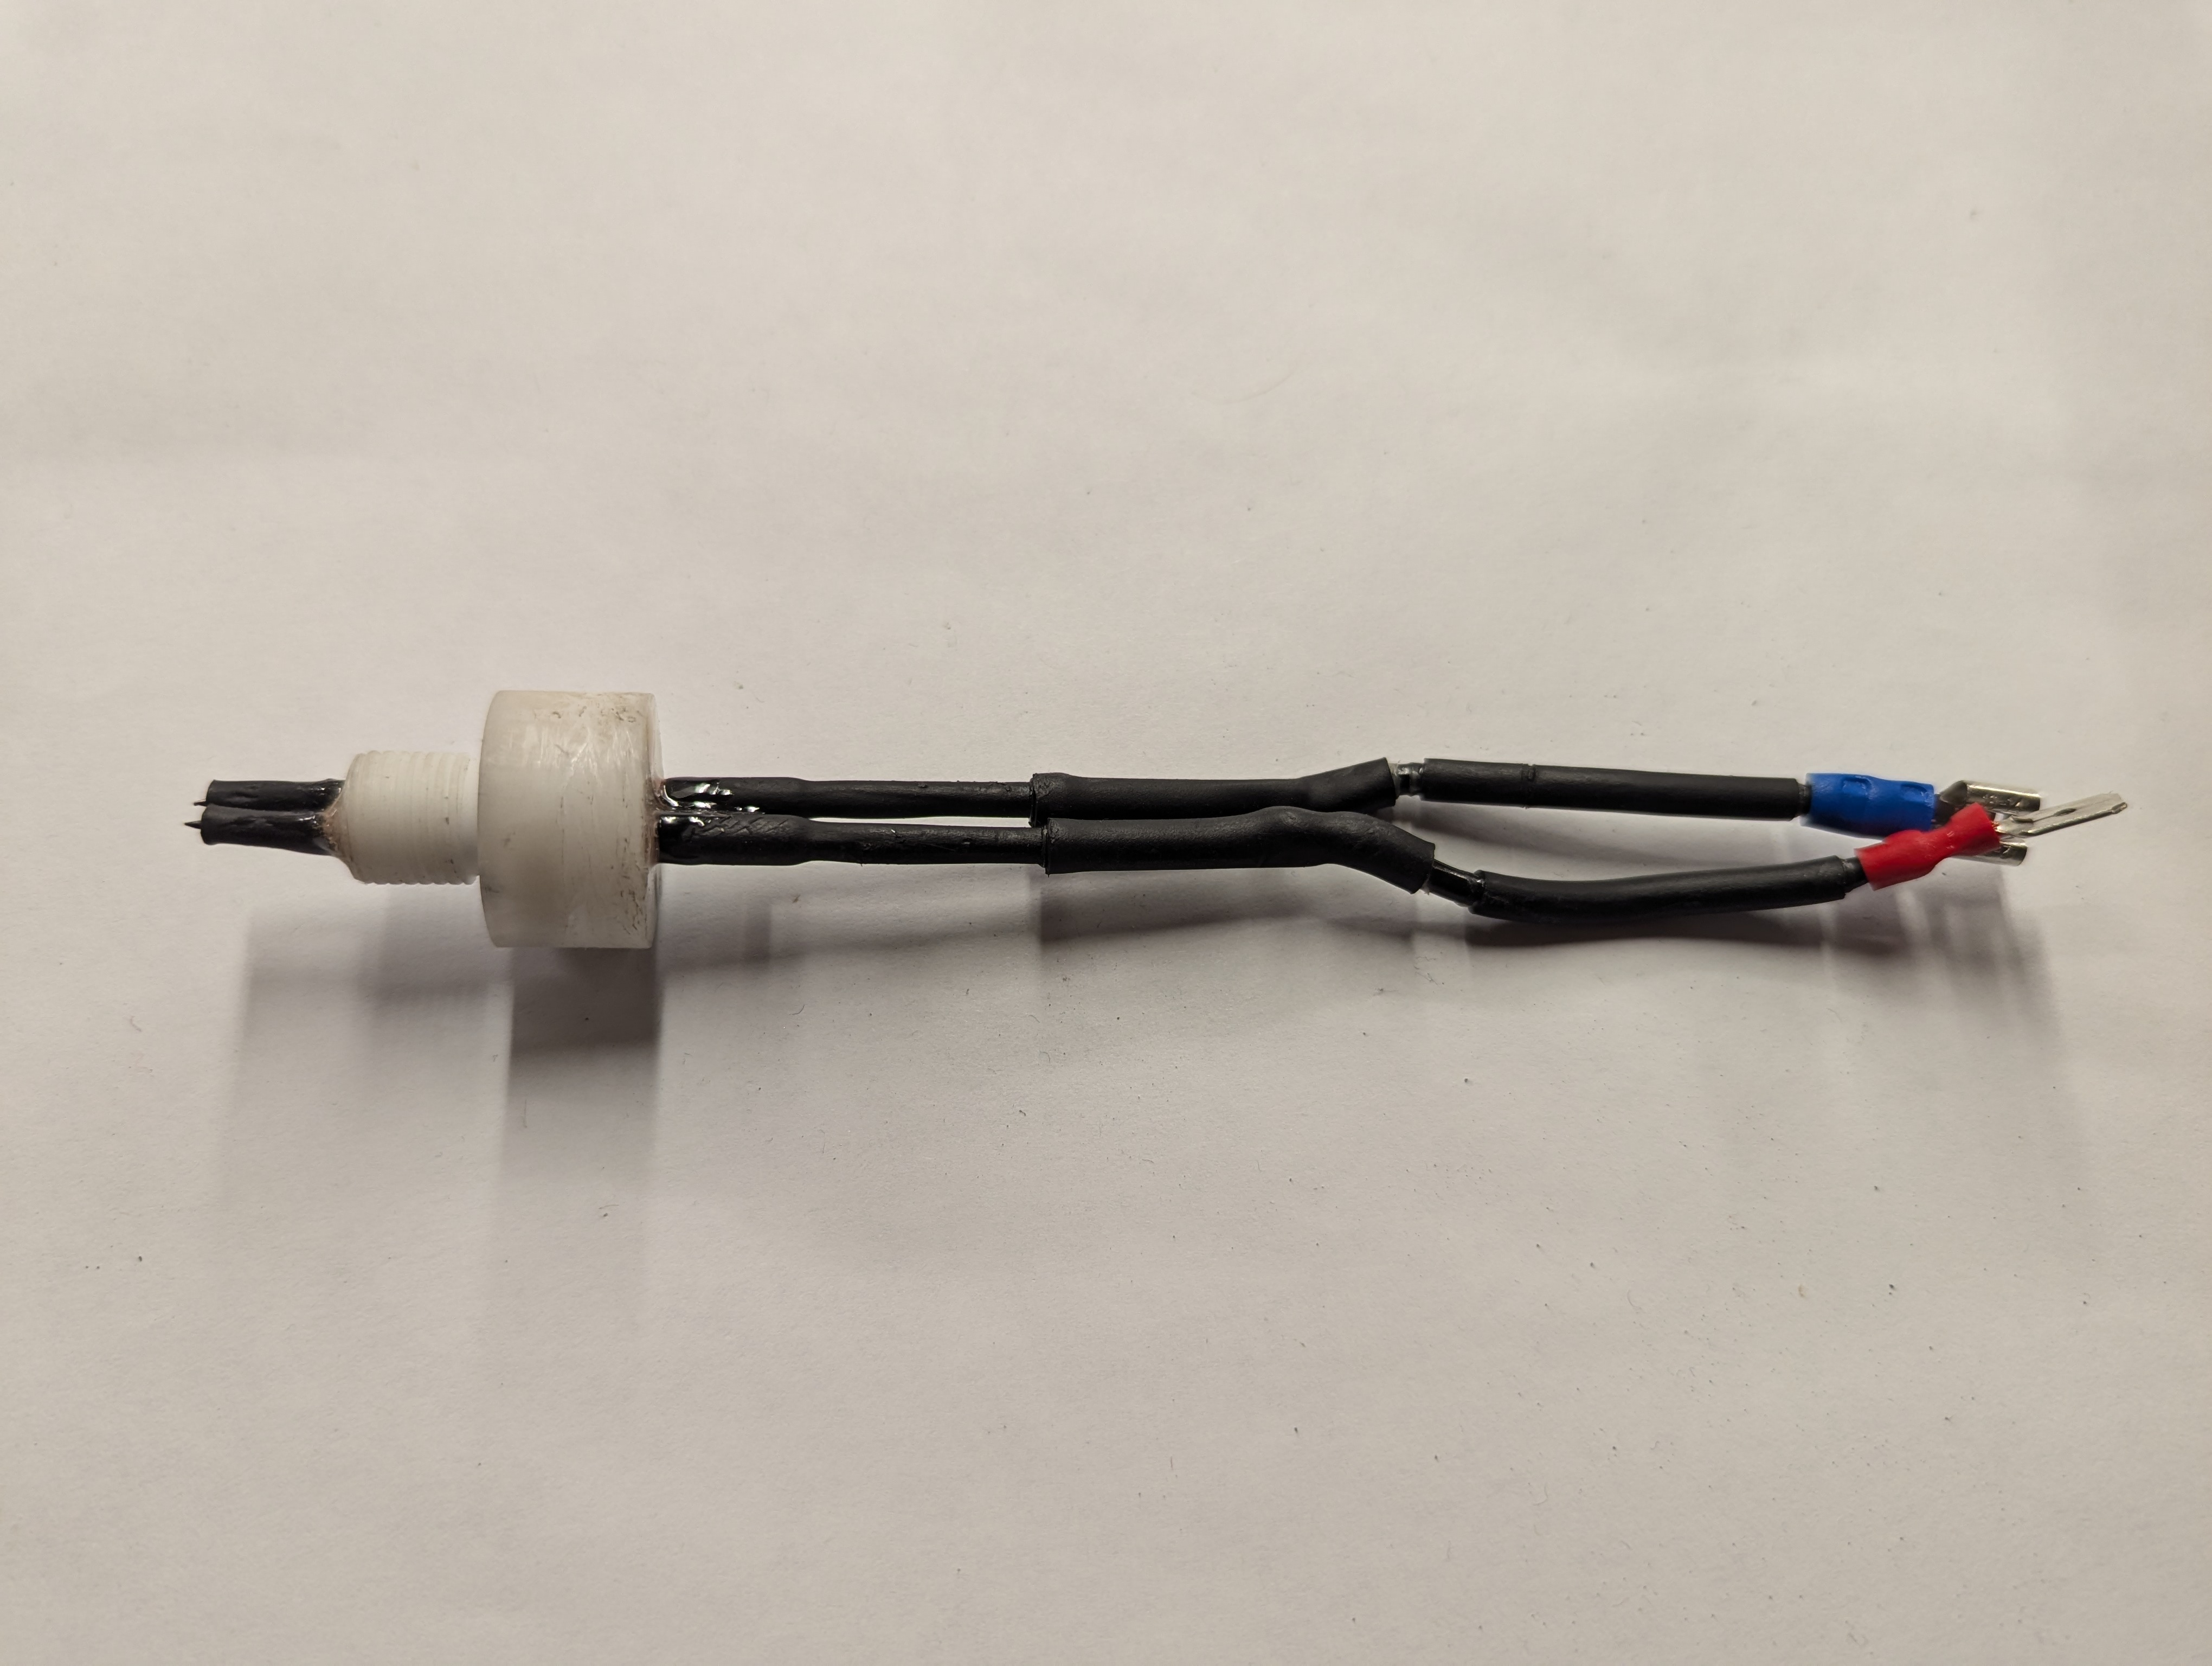
\includegraphics[width=0.5\textwidth]{assets/5 discussion/V1 single plug electrode.jpg}
    \caption{V1 single plug electrodes}
    \label{fig: V1 single plug electrodes}
\end{figure}

Using opposing electrodes would ensure that their tips were always the closest point to each other, greatly increasing spatial repeatability of the spark and enabling the electrode gap length to be easily adjusted. Opposing ports (\autoref{fig: V1 opposing ports}) were drilled into the bottom of the V1 apparatus to fit an electrode through the top and one through the bottom, as seen in \autoref{fig: standard view of electrodes}.

\begin{figure}[!ht]
    \centering
    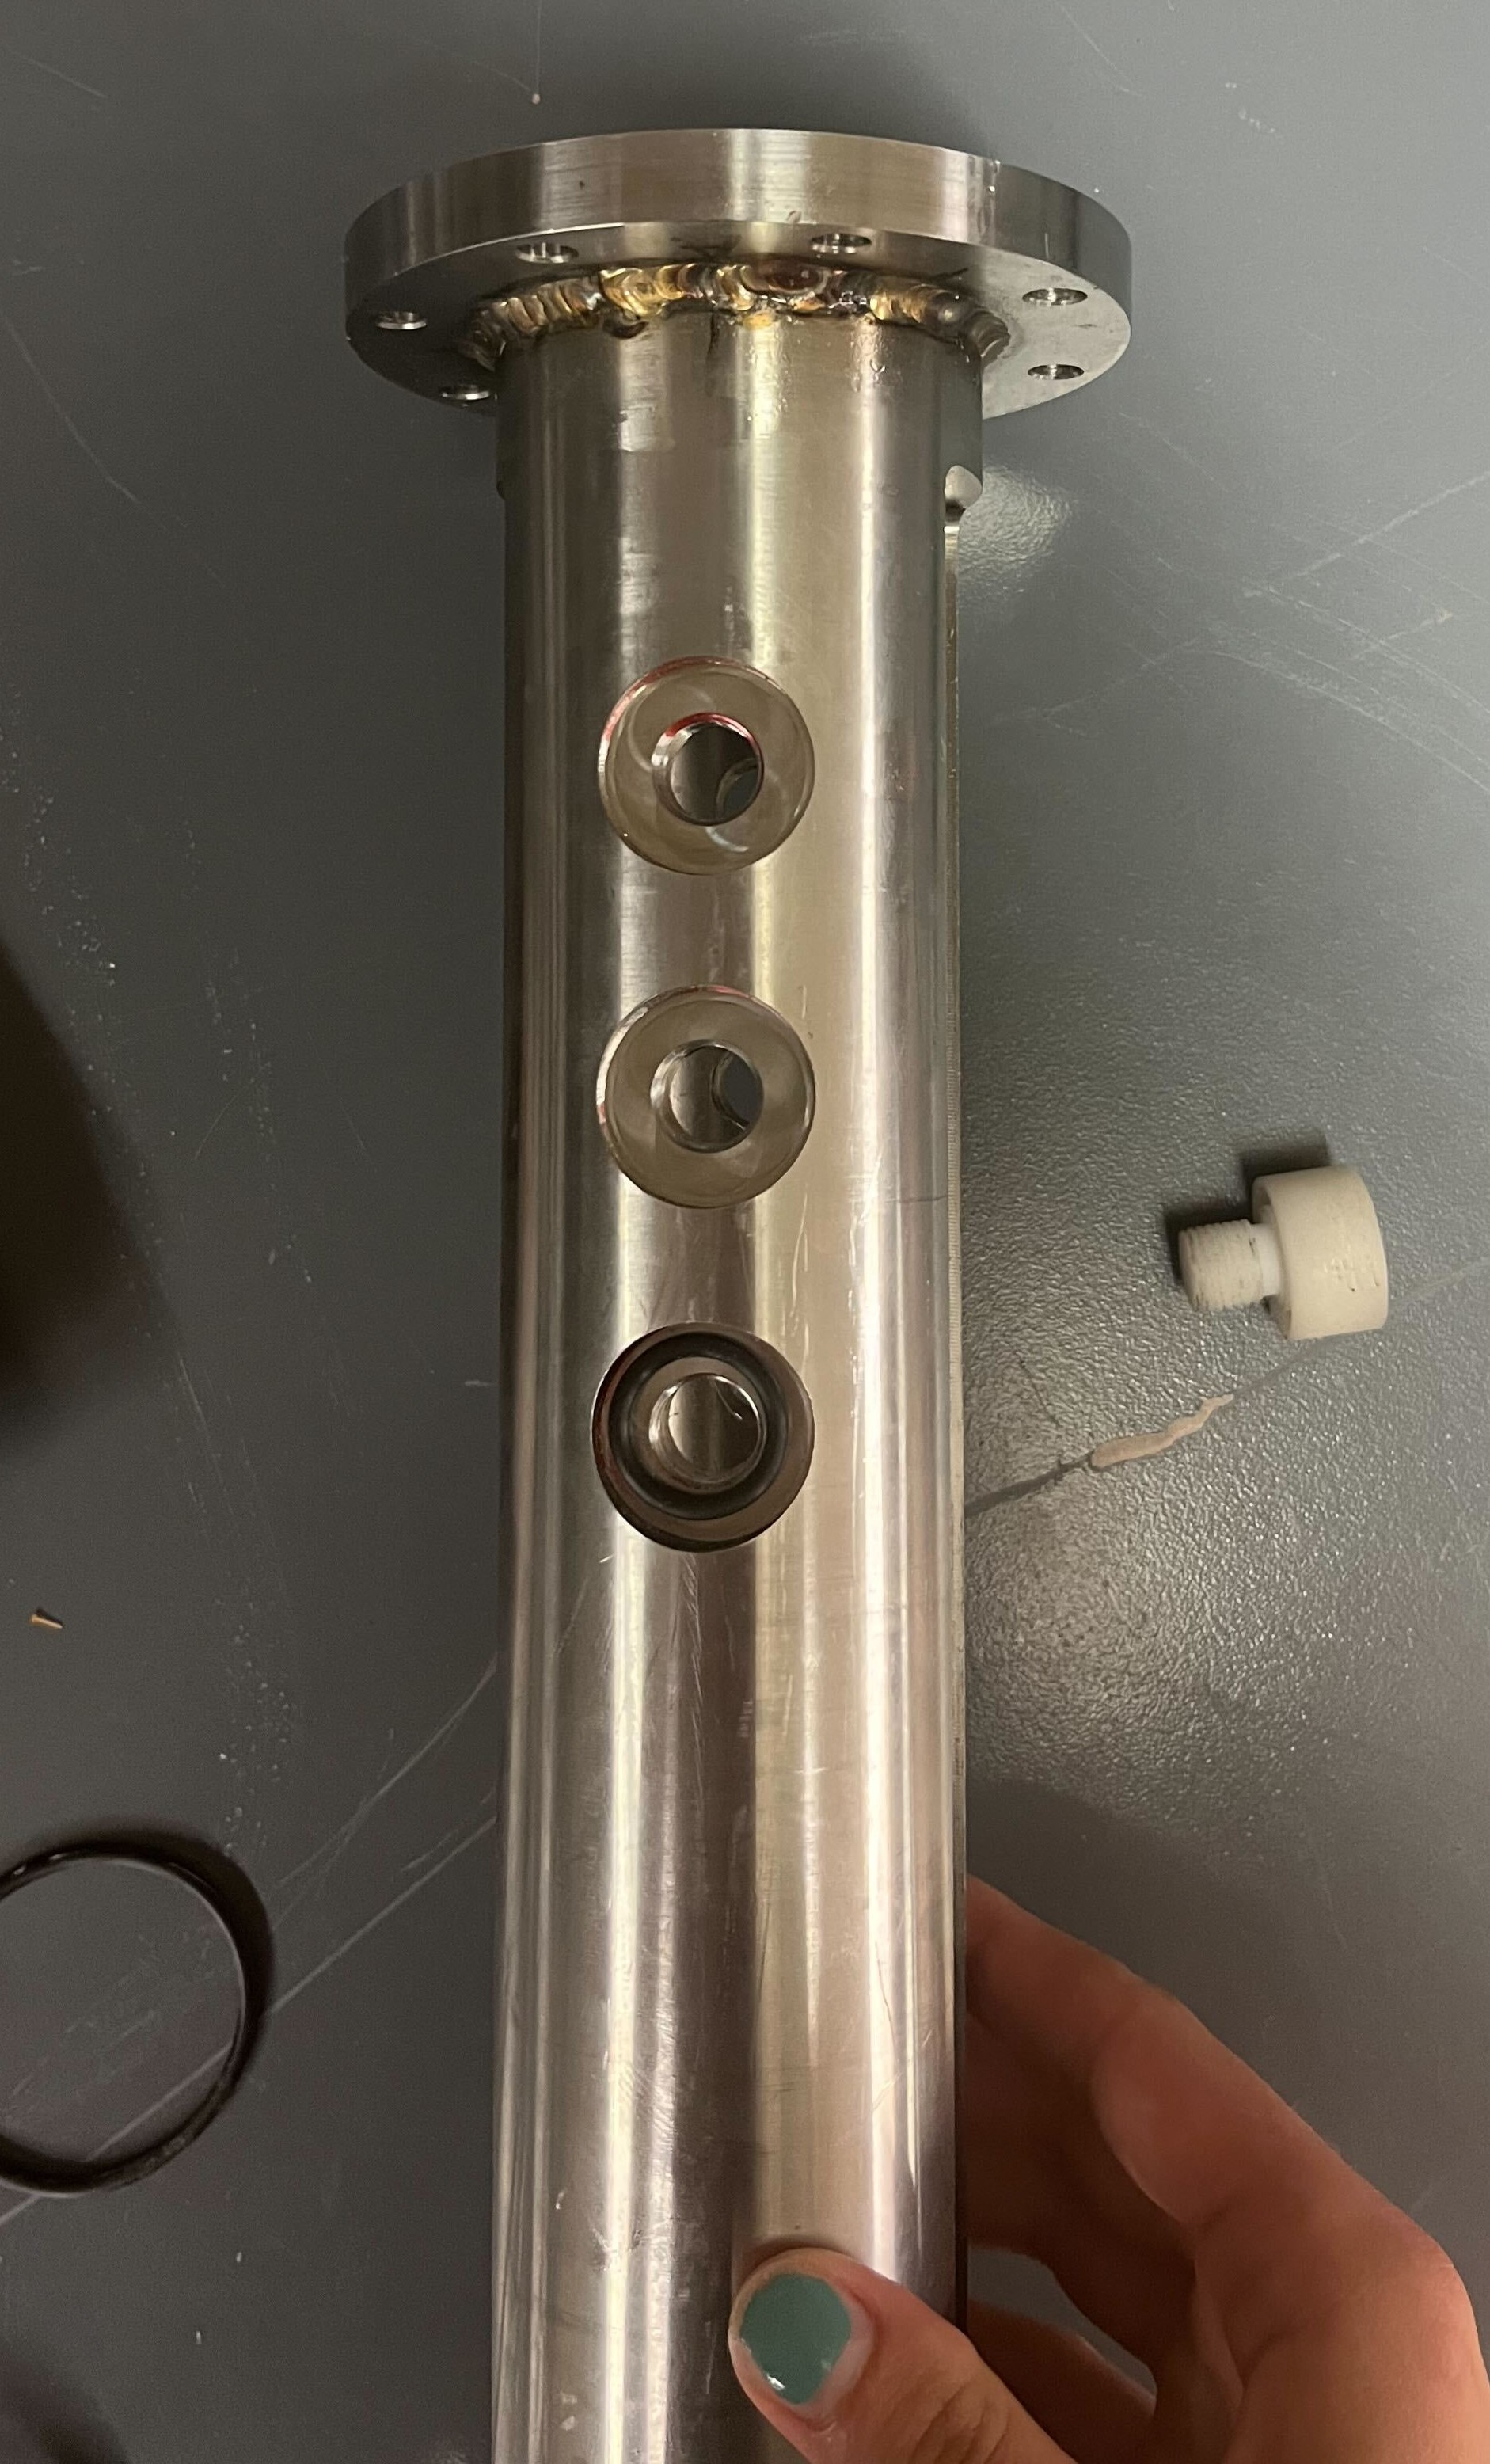
\includegraphics[width=0.5\textwidth]{assets/5 discussion/Bottom ports machined.jpg}
    \caption{V1 with newly machined opposing bottom ports}
    \label{fig: V1 opposing ports}
\end{figure}

% Coil burnout
Another critical issue was burnout of the automotive-type coils used in the spark initiation system. Five such coils were damaged to the point that they could no longer create a strong enough spark across the spark gap. A contributing factor could have been the poor electrode retention of the Ultra-Torr fittings, as \qty{20}{bar} of gas could visibly push the electrodes away \qtyrange{1}{2}{mm}. An increase in the spark gap increases its resistance, putting a higher load on the coil. Another concern was electromagnetic interference between the coil and its power supply. Originally in the same box, the \qty{10}{A} current-limited power supply and the smart coil were placed in separate electrical boxes (see \autoref{fig:Spark initiation}). Quad shielded coaxial cable was used between the coil and its controlling delay generator as an additional precaution. 

% V1 spark initiation! + Why was V2 designed?
Spatial alignment and timing synchronization of the laser focus to the spark was completed, and reliable spark initiation of LSP was achieved in V1. \ce{NO2} seeding tests were then undertaken to determine if more laser energy could be captured by the propellant. With as low as 0.6\% of \ce{NO2} partial pressure mixed with argon, double the pressure rise was observed. This indicated that the propellant was absorbing twice the energy from the plasma. As the \ce{NO2} fraction was increased, there were diminishing returns to the pressure rise. This was encouraging, as not much \ce{NO2} was needed to have a great impact on the energy absorption.

The V1 started showing downsides when it was being set up for thrust tests. Due to the weight of its steel construction, it created too much friction on its rails during cold flow thrust tests. This was mitigated in part by a rope system mentioned in \textcite{duplayArgonLaserPlasmaThruster2024a} but was not found to be repeatable. Having the LSP heat a smaller internal volume than the \qty{0.4}{L} of V1 was also desirable, as a greater effect on internal pressure and thrust would be seen. Critically, rubber seals were exposed to the laser path during continuous (CW) lasing with a lower focal length lens, severely melting them in the only V1 CW test conducted. A shorter test section designed for a \qty{100}{mm} focal length lens would allow the beam to pass through without hitting the sides of the test section. A smaller purpose-built test section, named V2, was therefore designed.

% Got V2 from capstone team
The achievement of consistent spark initiation with V1 coincided with the arrival of the V2 test section parts. Proof pressure testing of V2 up to \qty{75}{bar} for \qty{25}{minutes} was completed successfully. Unfortunately, the off-the-shelf \qty{44}{kV} wire originally intended to be used as the electrodes burst during pressure tests. An electrode redesign was therefore necessary. Molded dielectric epoxy (Stycast ES 1001 from McMasterCarr \autocite{McMasterCarr}) around an industrial sewing needle core was chosen, as it was economical and the outer diameter of the electrodes could be precisely controlled by sanding the surface of the set epoxy. Molds were 3D printed and Mann Ease Release\texttrademark 300 was applied to all their inside surfaces.

\begin{figure}[!ht]
    \centering
    \begin{subfigure}[t]{0.30\textwidth}
        \centering
        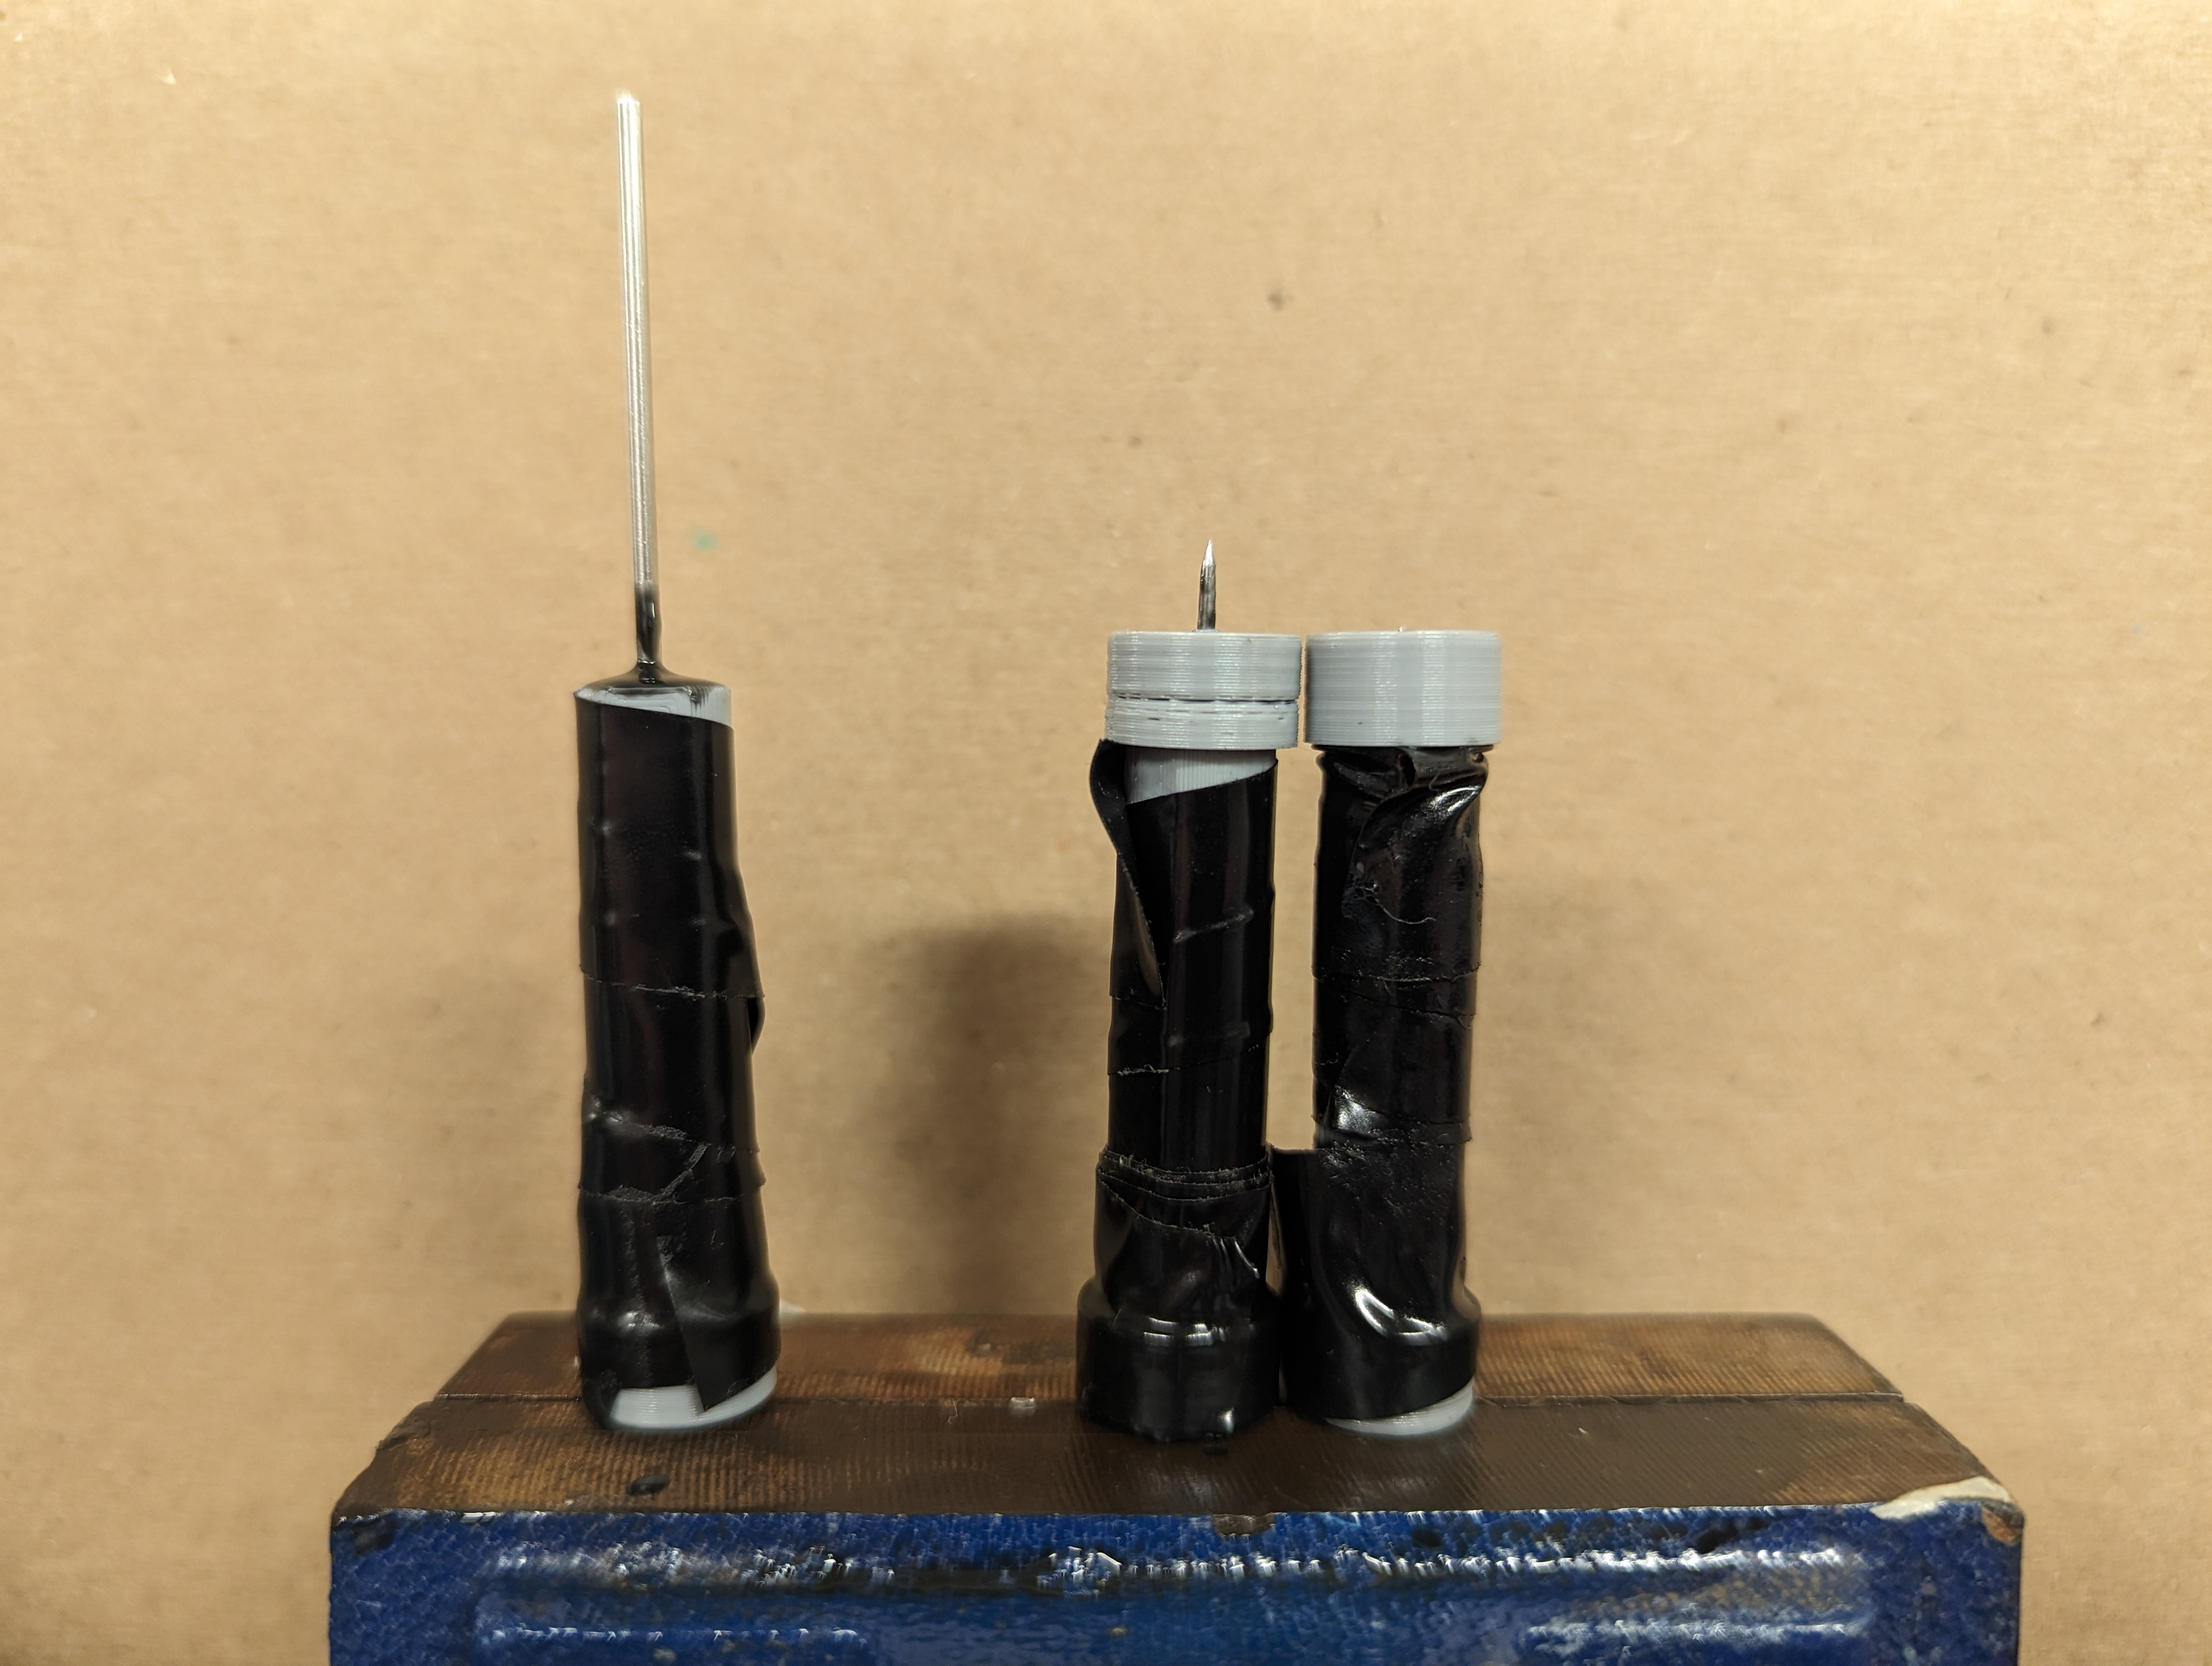
\includegraphics[width=\textwidth]{assets/3 design/Molds.jpg}
        \caption{Molds with steel needle core in place}
    \end{subfigure}
    \hfill
    \begin{subfigure}[t]{0.30\textwidth}
        \centering
        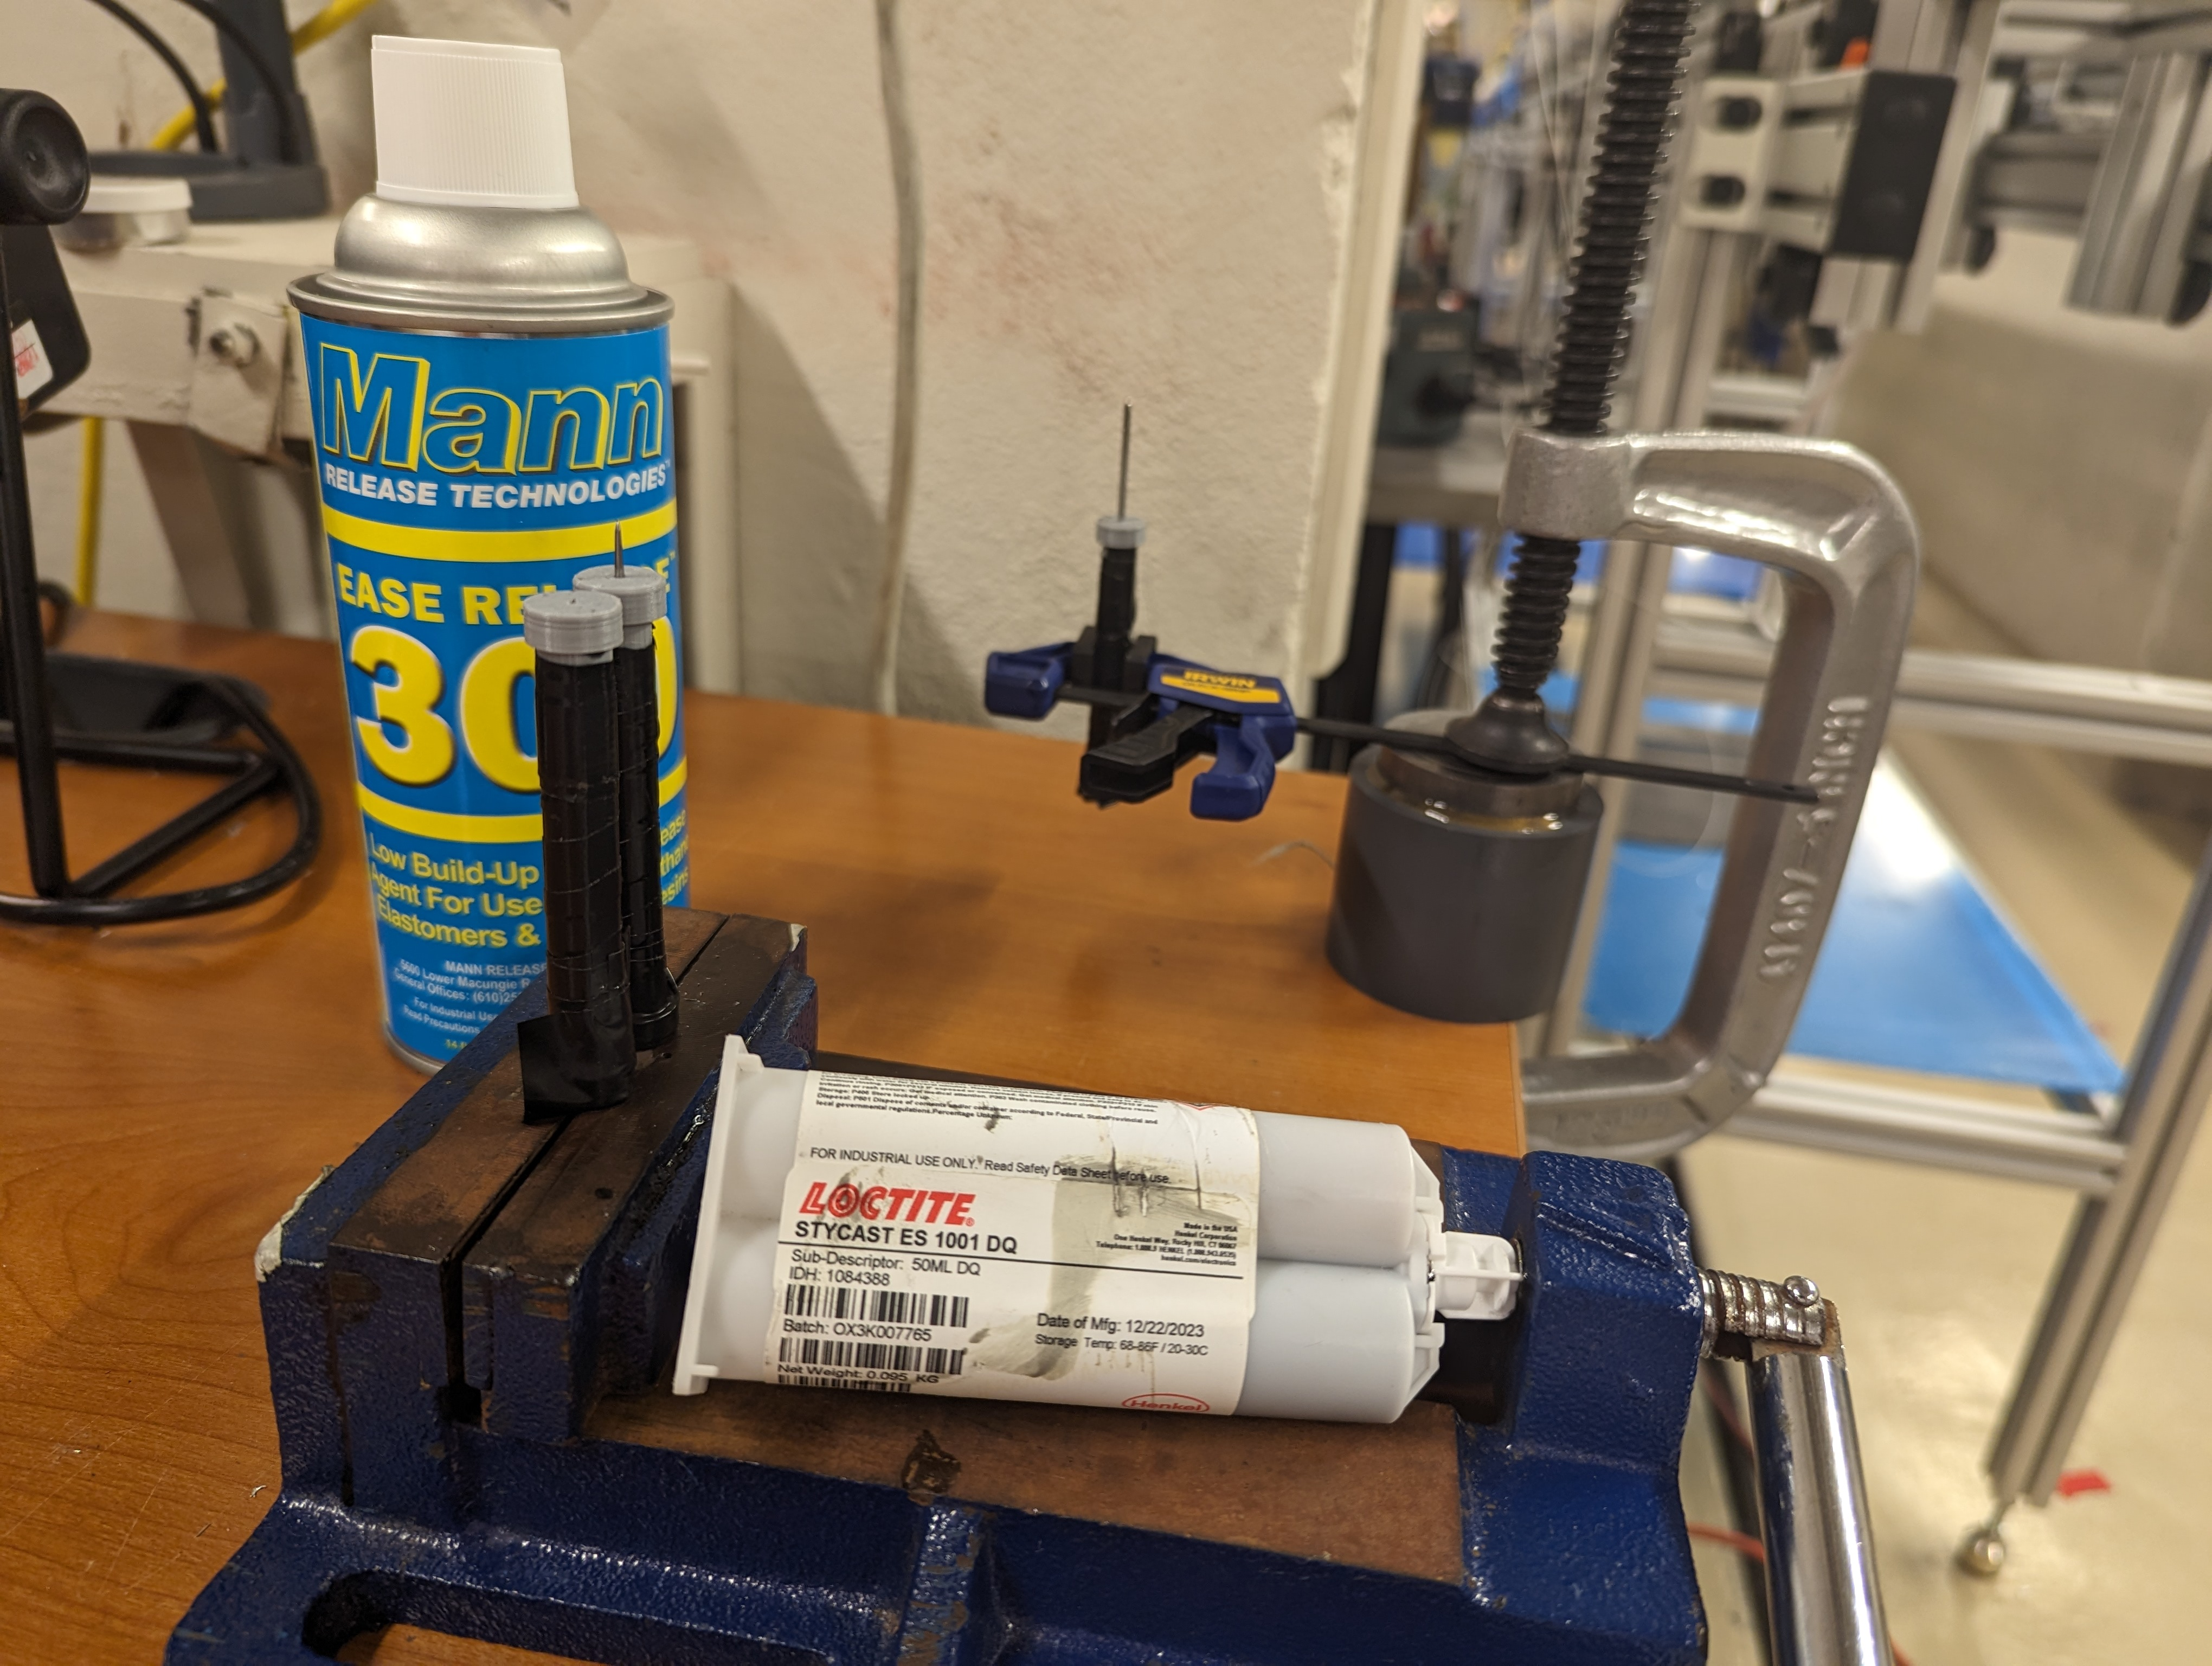
\includegraphics[width=\textwidth]{assets/3 design/Mold process.jpg}
        \caption{Molding process}
    \end{subfigure}
    \hfill
    \begin{subfigure}[t]{0.30\textwidth}
        \centering
        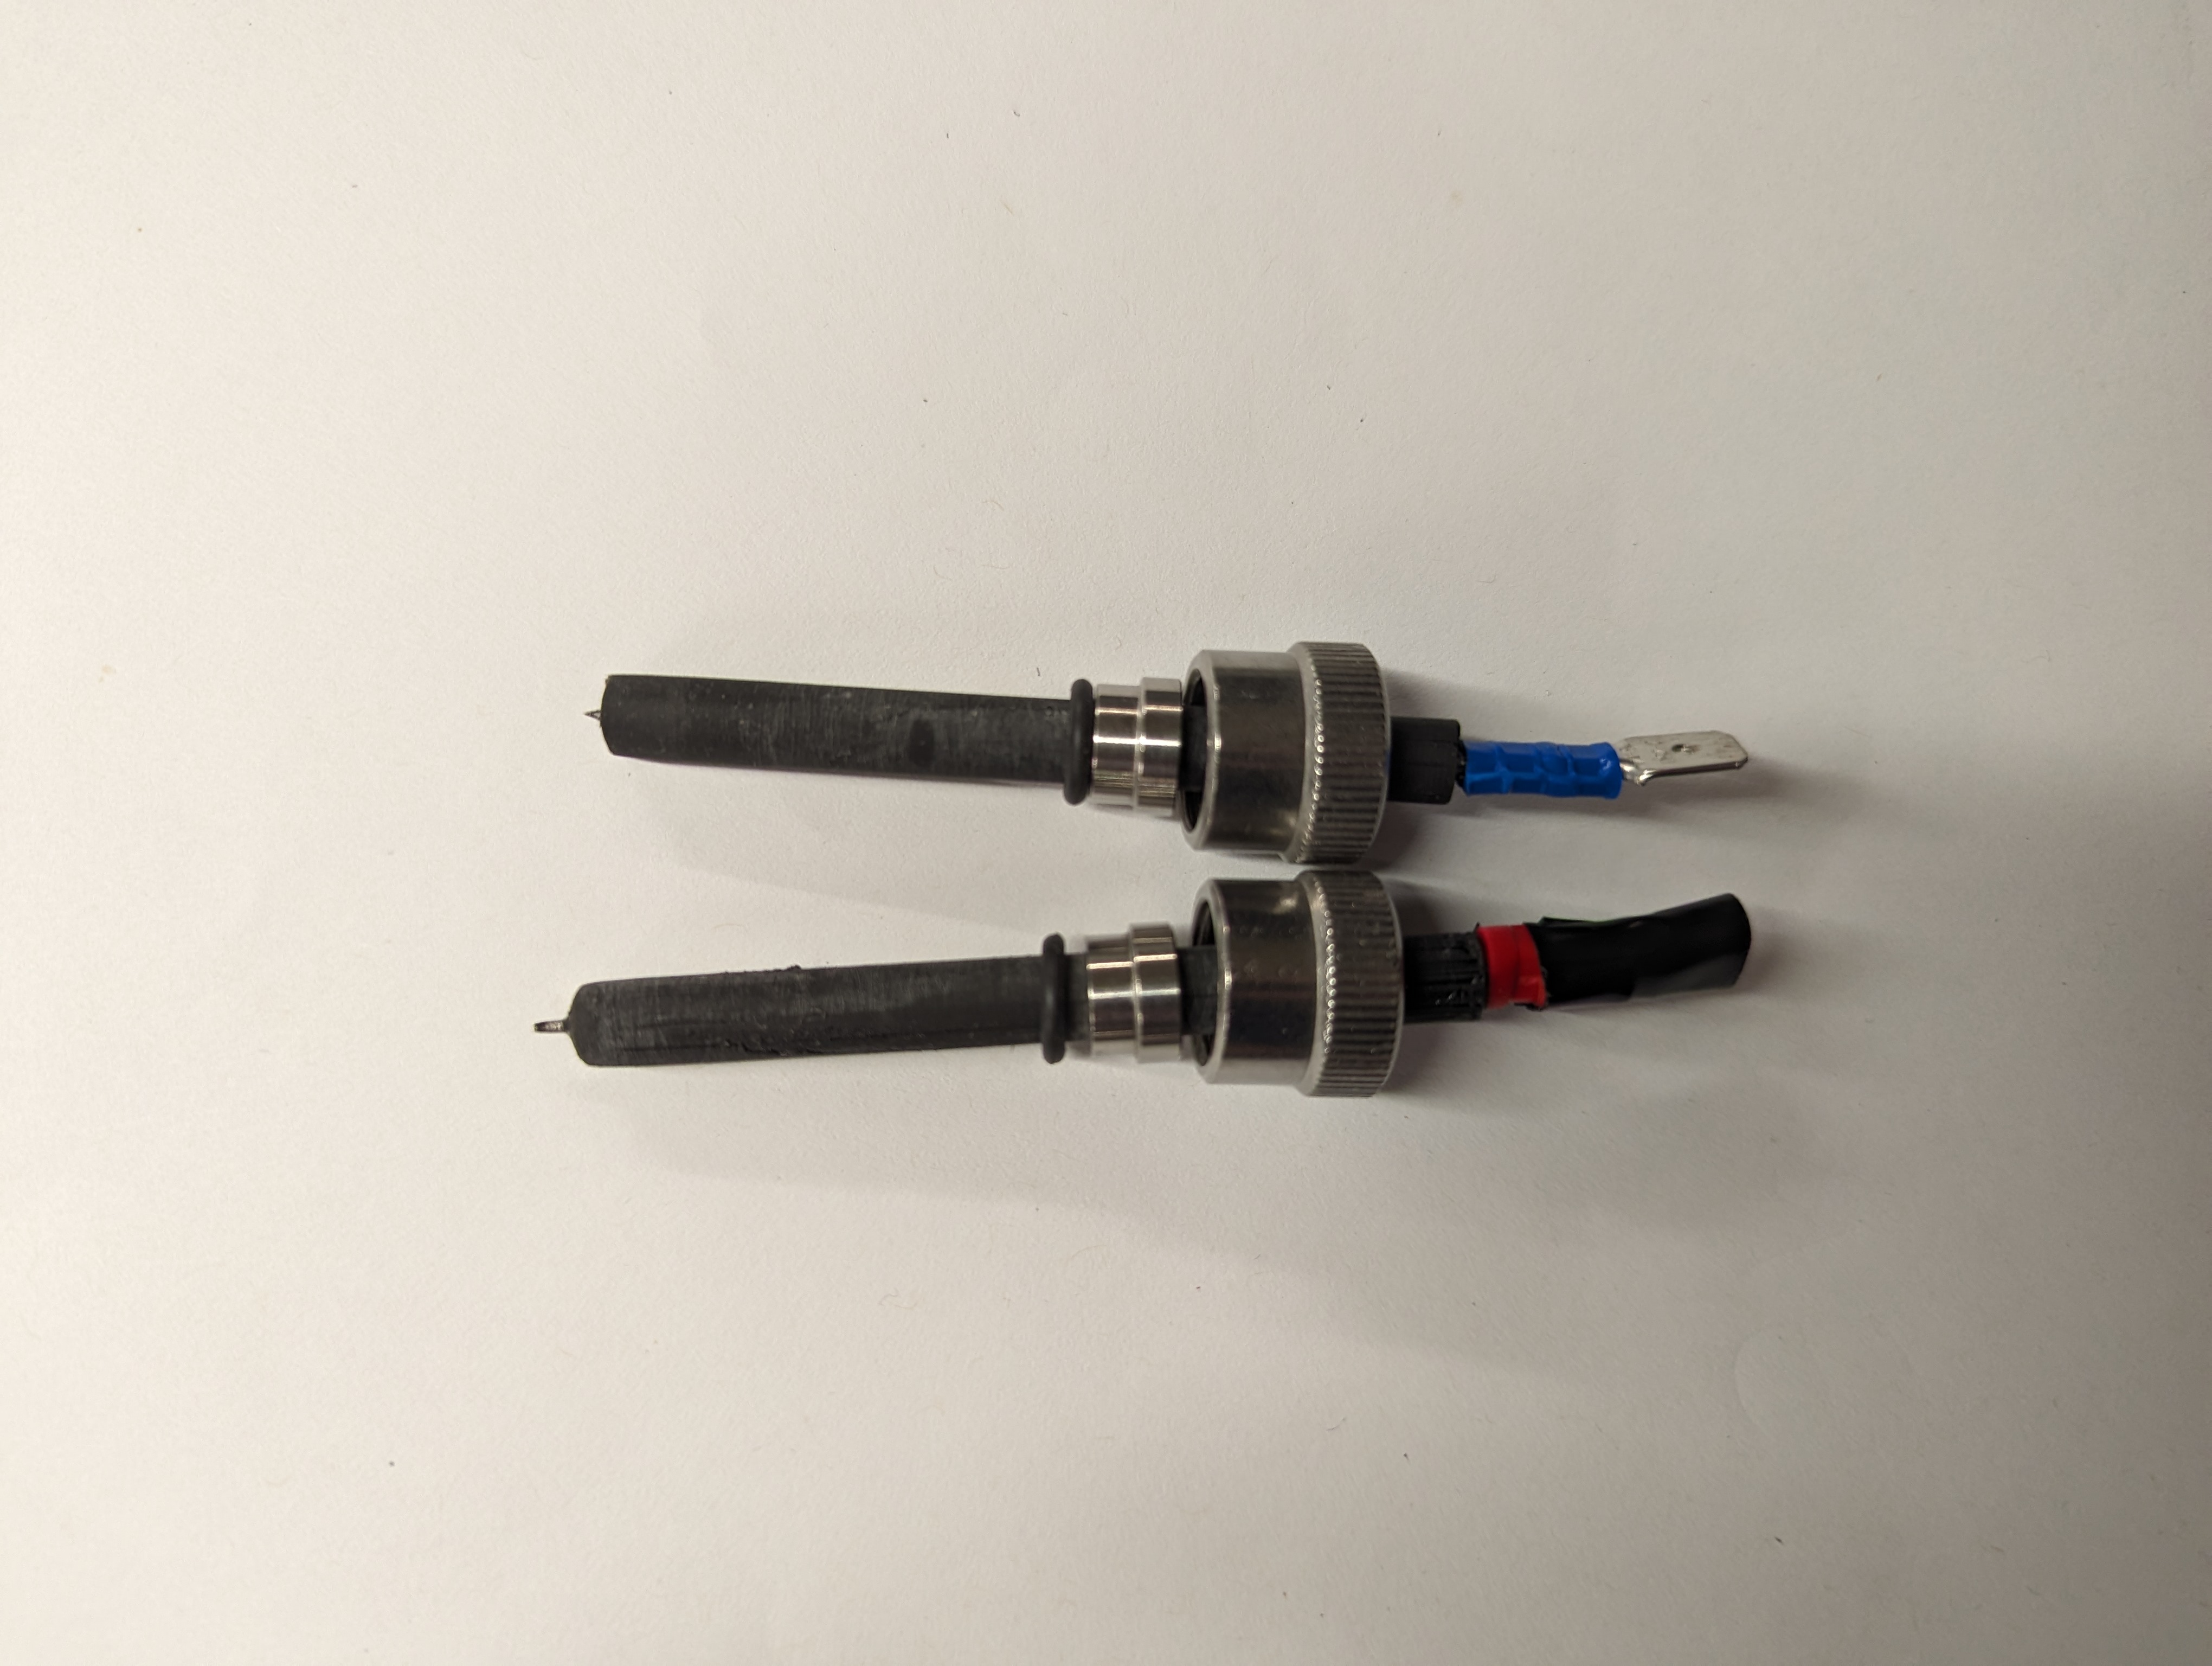
\includegraphics[width=\textwidth]{assets/3 design/V2 electrodes.jpg}
        \caption{Assembled electrodes with Ultra-Torr cap and electrical connectors}
        \label{fig:Assembled electrode}
    \end{subfigure}

    \caption{Electrode manufacturing process}
\end{figure}

The electrodes were then sanded down to fit tightly into Ultra-Torr vacuum connectors. Although these connectors were not designed for high pressure, previous experience has shown that they are appropriate up to about \qty{20}{bar} if tightened enough. The result is presented in \autoref{fig:Assembled electrode}. Once installed in the V2 thruster, the electrodes were pushed into contact with each other and the Ultra-Torr connectors tightened. Statically pressurizing V2 to \qty{20}{bar} was enough to separate the electrodes from one another by about \qty{1}{mm}.

With a dual-lens system, static LSP via spark initiation in V2 was achieved on the first QCW shot at 100\% power (\qty{3079}{W}). This was initially done with a flat aluminum plate at the end of the test section (see \autoref{fig:initial V2 static config} and \autoref{chp:V2 Test Section Drawings}). 

\begin{figure}[!ht]
    \centering
    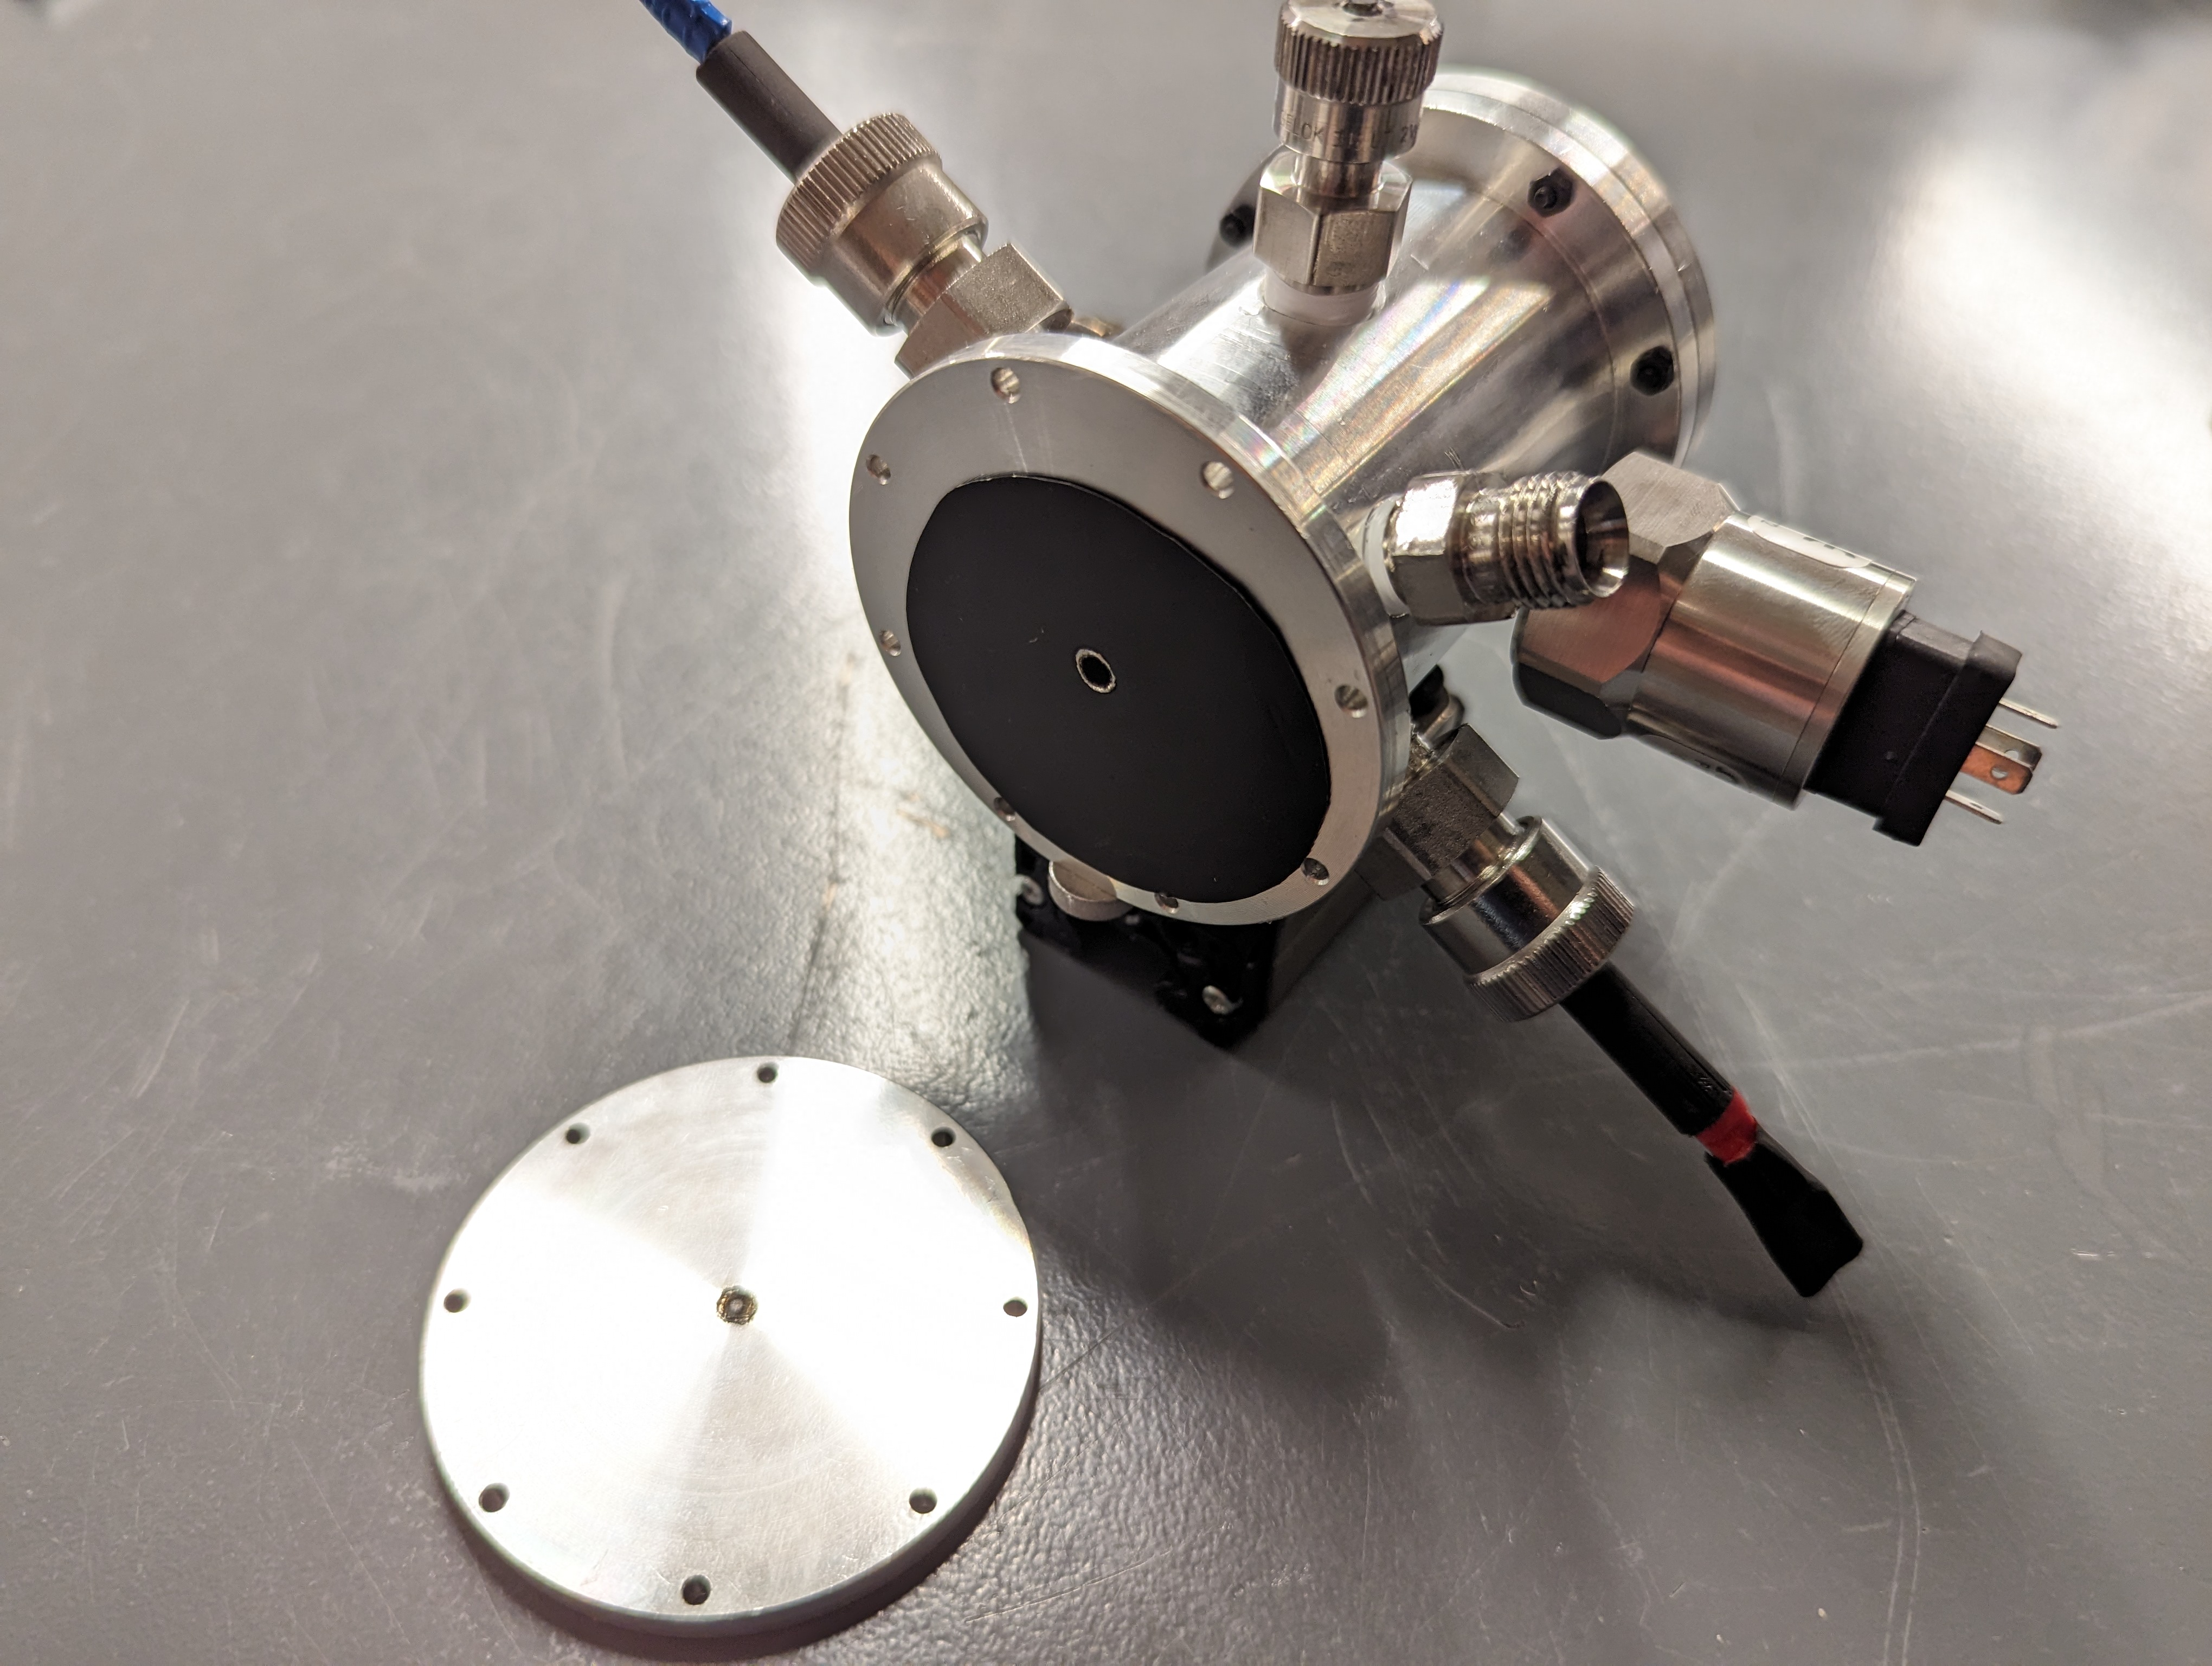
\includegraphics[width=0.45\textwidth]{assets/4 experiments/V2 test damage.jpg}
    \caption{Ablation damage to the flat rear plate of the thruster after two \qty{3}{kW} laser shots}
    \label{fig:initial V2 static config}
\end{figure}

The black sheet in \autoref{fig:initial V2 static config} is Thorlabs laser-absorbing aluminum foil, used in a failed attempt to protect the rear plate from damage. In addition to this ablation problem, the laser could only be aligned between the electrodes when the rear plate was taken off. This required re-pressurization after every attempt at alignment. Given that the electrodes would also move under the \qty{20}{bar} pressure, this was very tedious. 

To solve this, a second window holder was machined (\autoref{chp:V2 rear window mount}) to replace the flat plate. The laser could then be aligned when the test section was pressurized, and the alignment could be changed without opening the thruster. The window allowed the laser energy that was not absorbed by the plasma to pass freely through the apparatus, also enabling power meter measurements. With the new window mount installed, the goal was then to bring the QCW initiation power down to the maximum CW power of the laser, \qty{342}{W}, in order to attempt a CW LSP.

% Discussion on acheivement of V2 CW LSP:
A dual-lens system was designed to increase laser flux at the focus by decreasing the area of the focus while keeping the power constant. The lenses were validated with V1 and used in all of V2's LSP shots. Once LSPs lower than \qty{342}{W} were initiated reliably, our first 100\% power (\qty{342}{W}) CW LSP was generated for \qty{85.1}{ms}, a 1.7 times longer lifetime than the maximum QCW pulse length of \qty{50.0}{ms}. While these results were encouraging, more experiments with CW laser operation must be completed to determine if lifetimes can be extended to an order of magnitude more, i.e. around one second. This would help with measuring a difference in thrust when the laser is on, as the energy transmitted to the gas would also be increased by the same amount.

% Damage to window and extension tube
After the first CW LSP, more CW and pulsed shots were attempted. These continued to damage the rear window, as seen in the center of \autoref{fig:Rear window damage}. Eventually, a \qty{3}{s} CW shot melted it severely enough that visual laser alignment between the electrodes of V2 was no longer possible.
\begin{figure}[!ht]
    \centering
    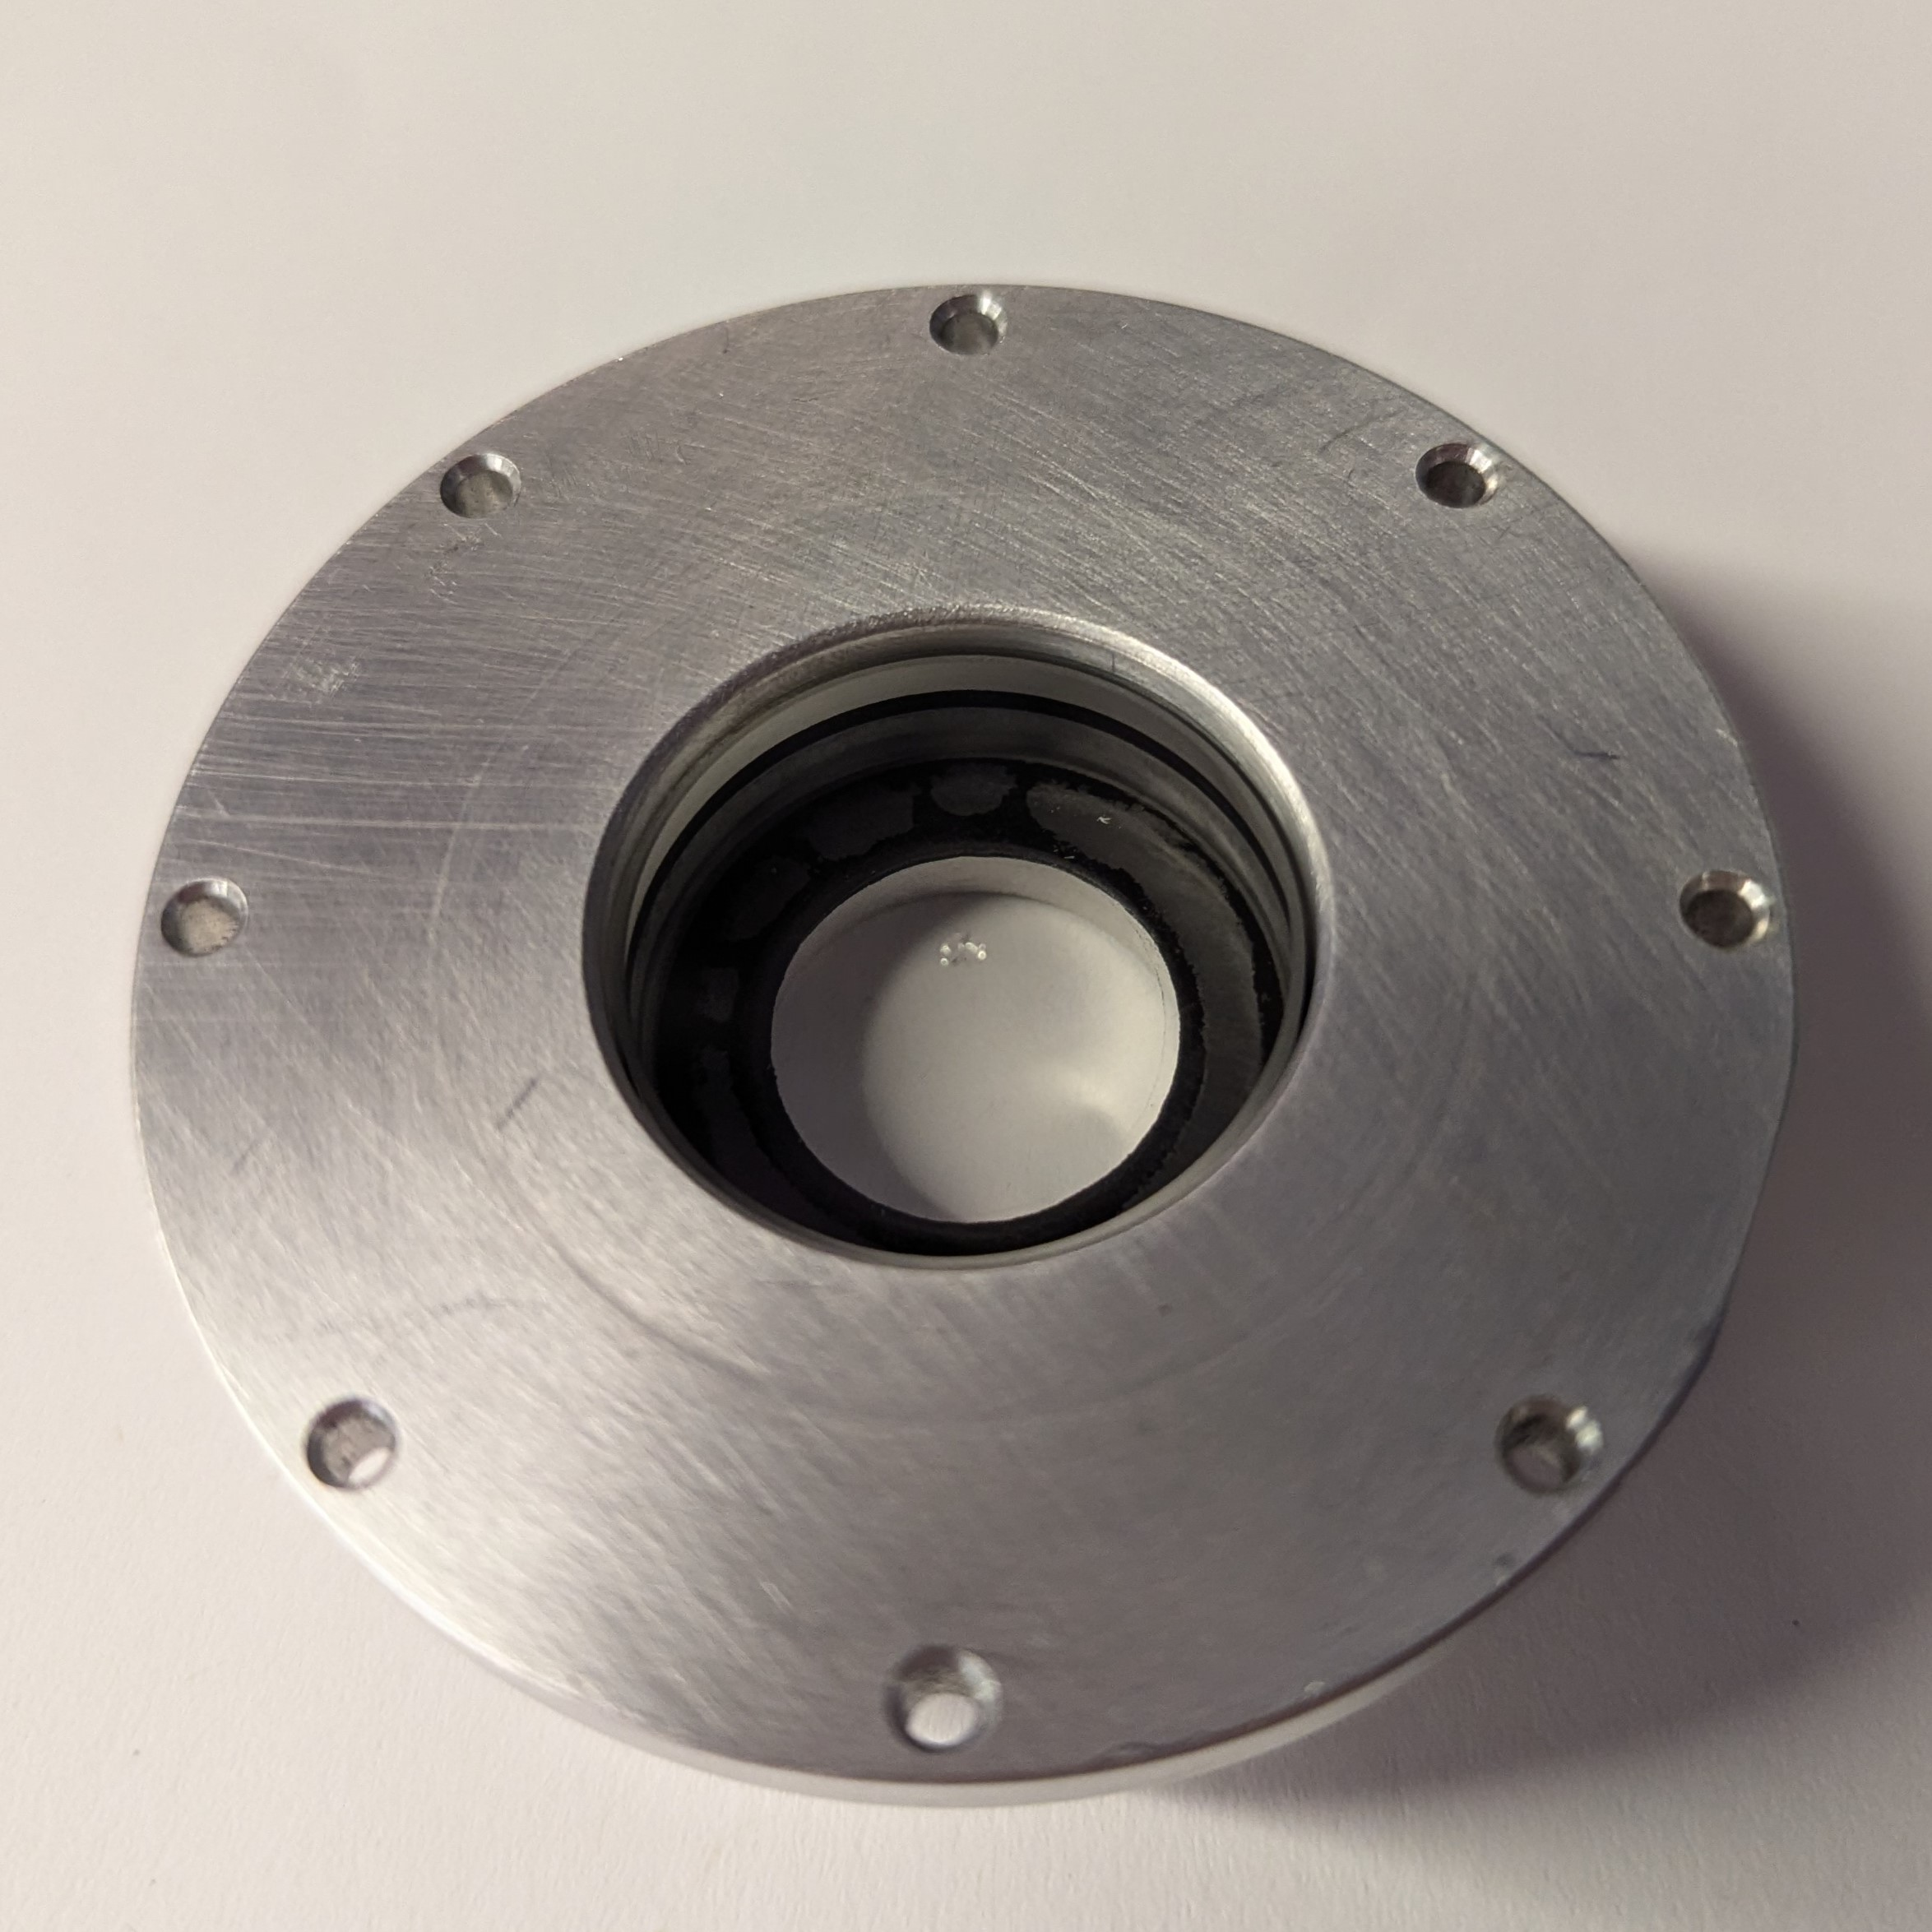
\includegraphics[width=0.45\textwidth]{assets/4 experiments/window damage.jpg}
    \caption{Rear window damage on V2}
    \label{fig:Rear window damage}
\end{figure}
A window extension tube (seen in \autoref{fig: window extension tube}, drawings in \autoref{chp:Extension cylinder}) was manufactured to solve this, moving the rear window downstream to where the laser flux was comparable to the front window, where no damage was seen. This extension tube has yet to be tested.
\begin{figure}[!ht]
    \centering
    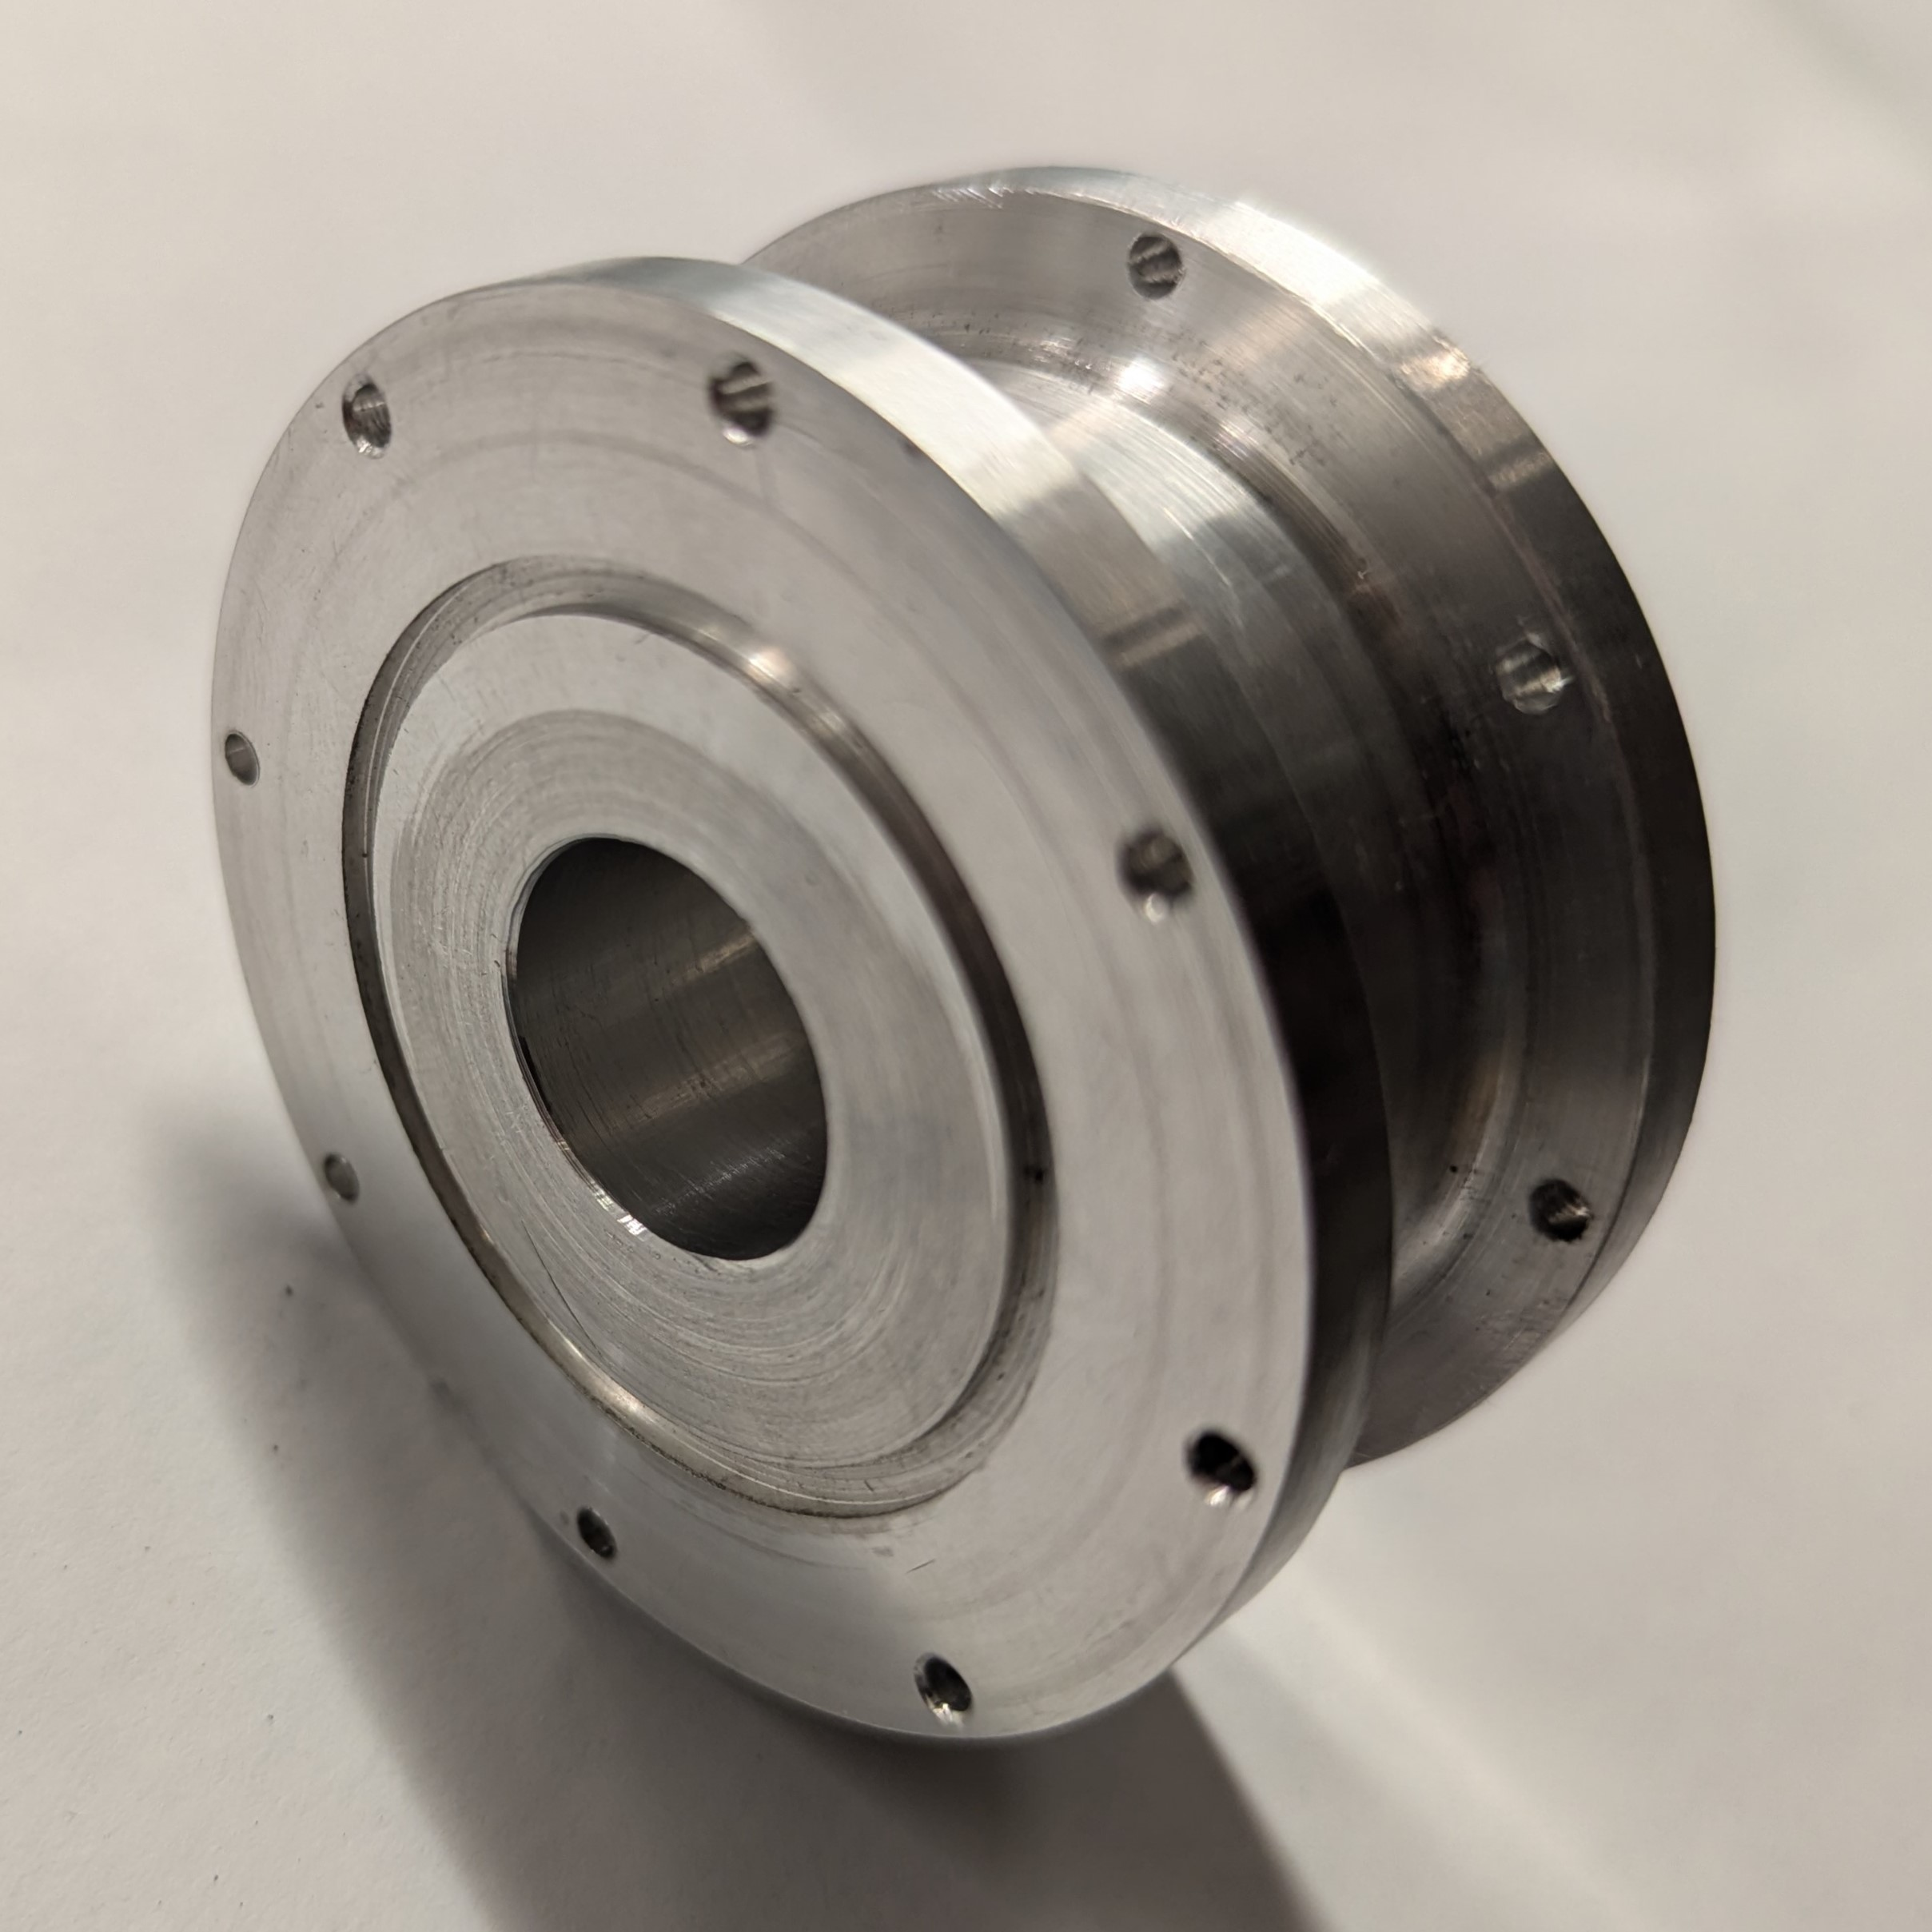
\includegraphics[width=0.45\textwidth]{assets/5 discussion/Extension cylinder.jpg}
    \caption{Window extension tube}
    \label{fig: window extension tube}
\end{figure}

% Cold flow thruster characterisation, hysterisis discussion
In parallel to the static LSP validation, characterization of the thruster with argon cold flow was advanced. High hysteresis of the thrust measurements was found, with the thrust stand often not returning to its original zero after a cold flow test. To attempt to correct these problems, a more sensitive load cell was installed with a \qtyrange{0}{5}{N} force sensing range (Honeywell FSG005WNPB). Lubricant was also added to the cart's bearings. However, the hysteresis issue remained (see \autoref{fig:hysteresis}) due to high friction between the rail and the ball bearing carriage preventing the thruster from resetting at the same place every time. The present thrust stand is therefore inadequate for future thrust tests and a new one should be built to measure thrust repeatably and reliably.

% QCW LSP thrust tests with V2:
Initial QCW LSP (pulsed hot fire) thrust tests aimed to determine if QCW LSP initiated by a spark in flowing argon was possible with V2, and if usable thrust data could be collected. It was shown that LSP could be initiated, and a change of thrust was measured, but this was due to nozzle ablation in all cases. \autoref{fig:nozzle ablation} shows nozzle ablation during a QCW flowing test without LSP, with \autoref{fig:Nozzle laser damage} showing the damage to the nozzle afterward. No LSP was initiated in this test, however a plasma plume can be seen exiting the nozzle. This plasma was again generated by nozzle ablation, proving that this experiment can operate as a laser ablation thruster. This result was not what the thruster was designed for and lead to a redesign of the V2 nozzle.

\begin{figure}[!ht]
    \centering
    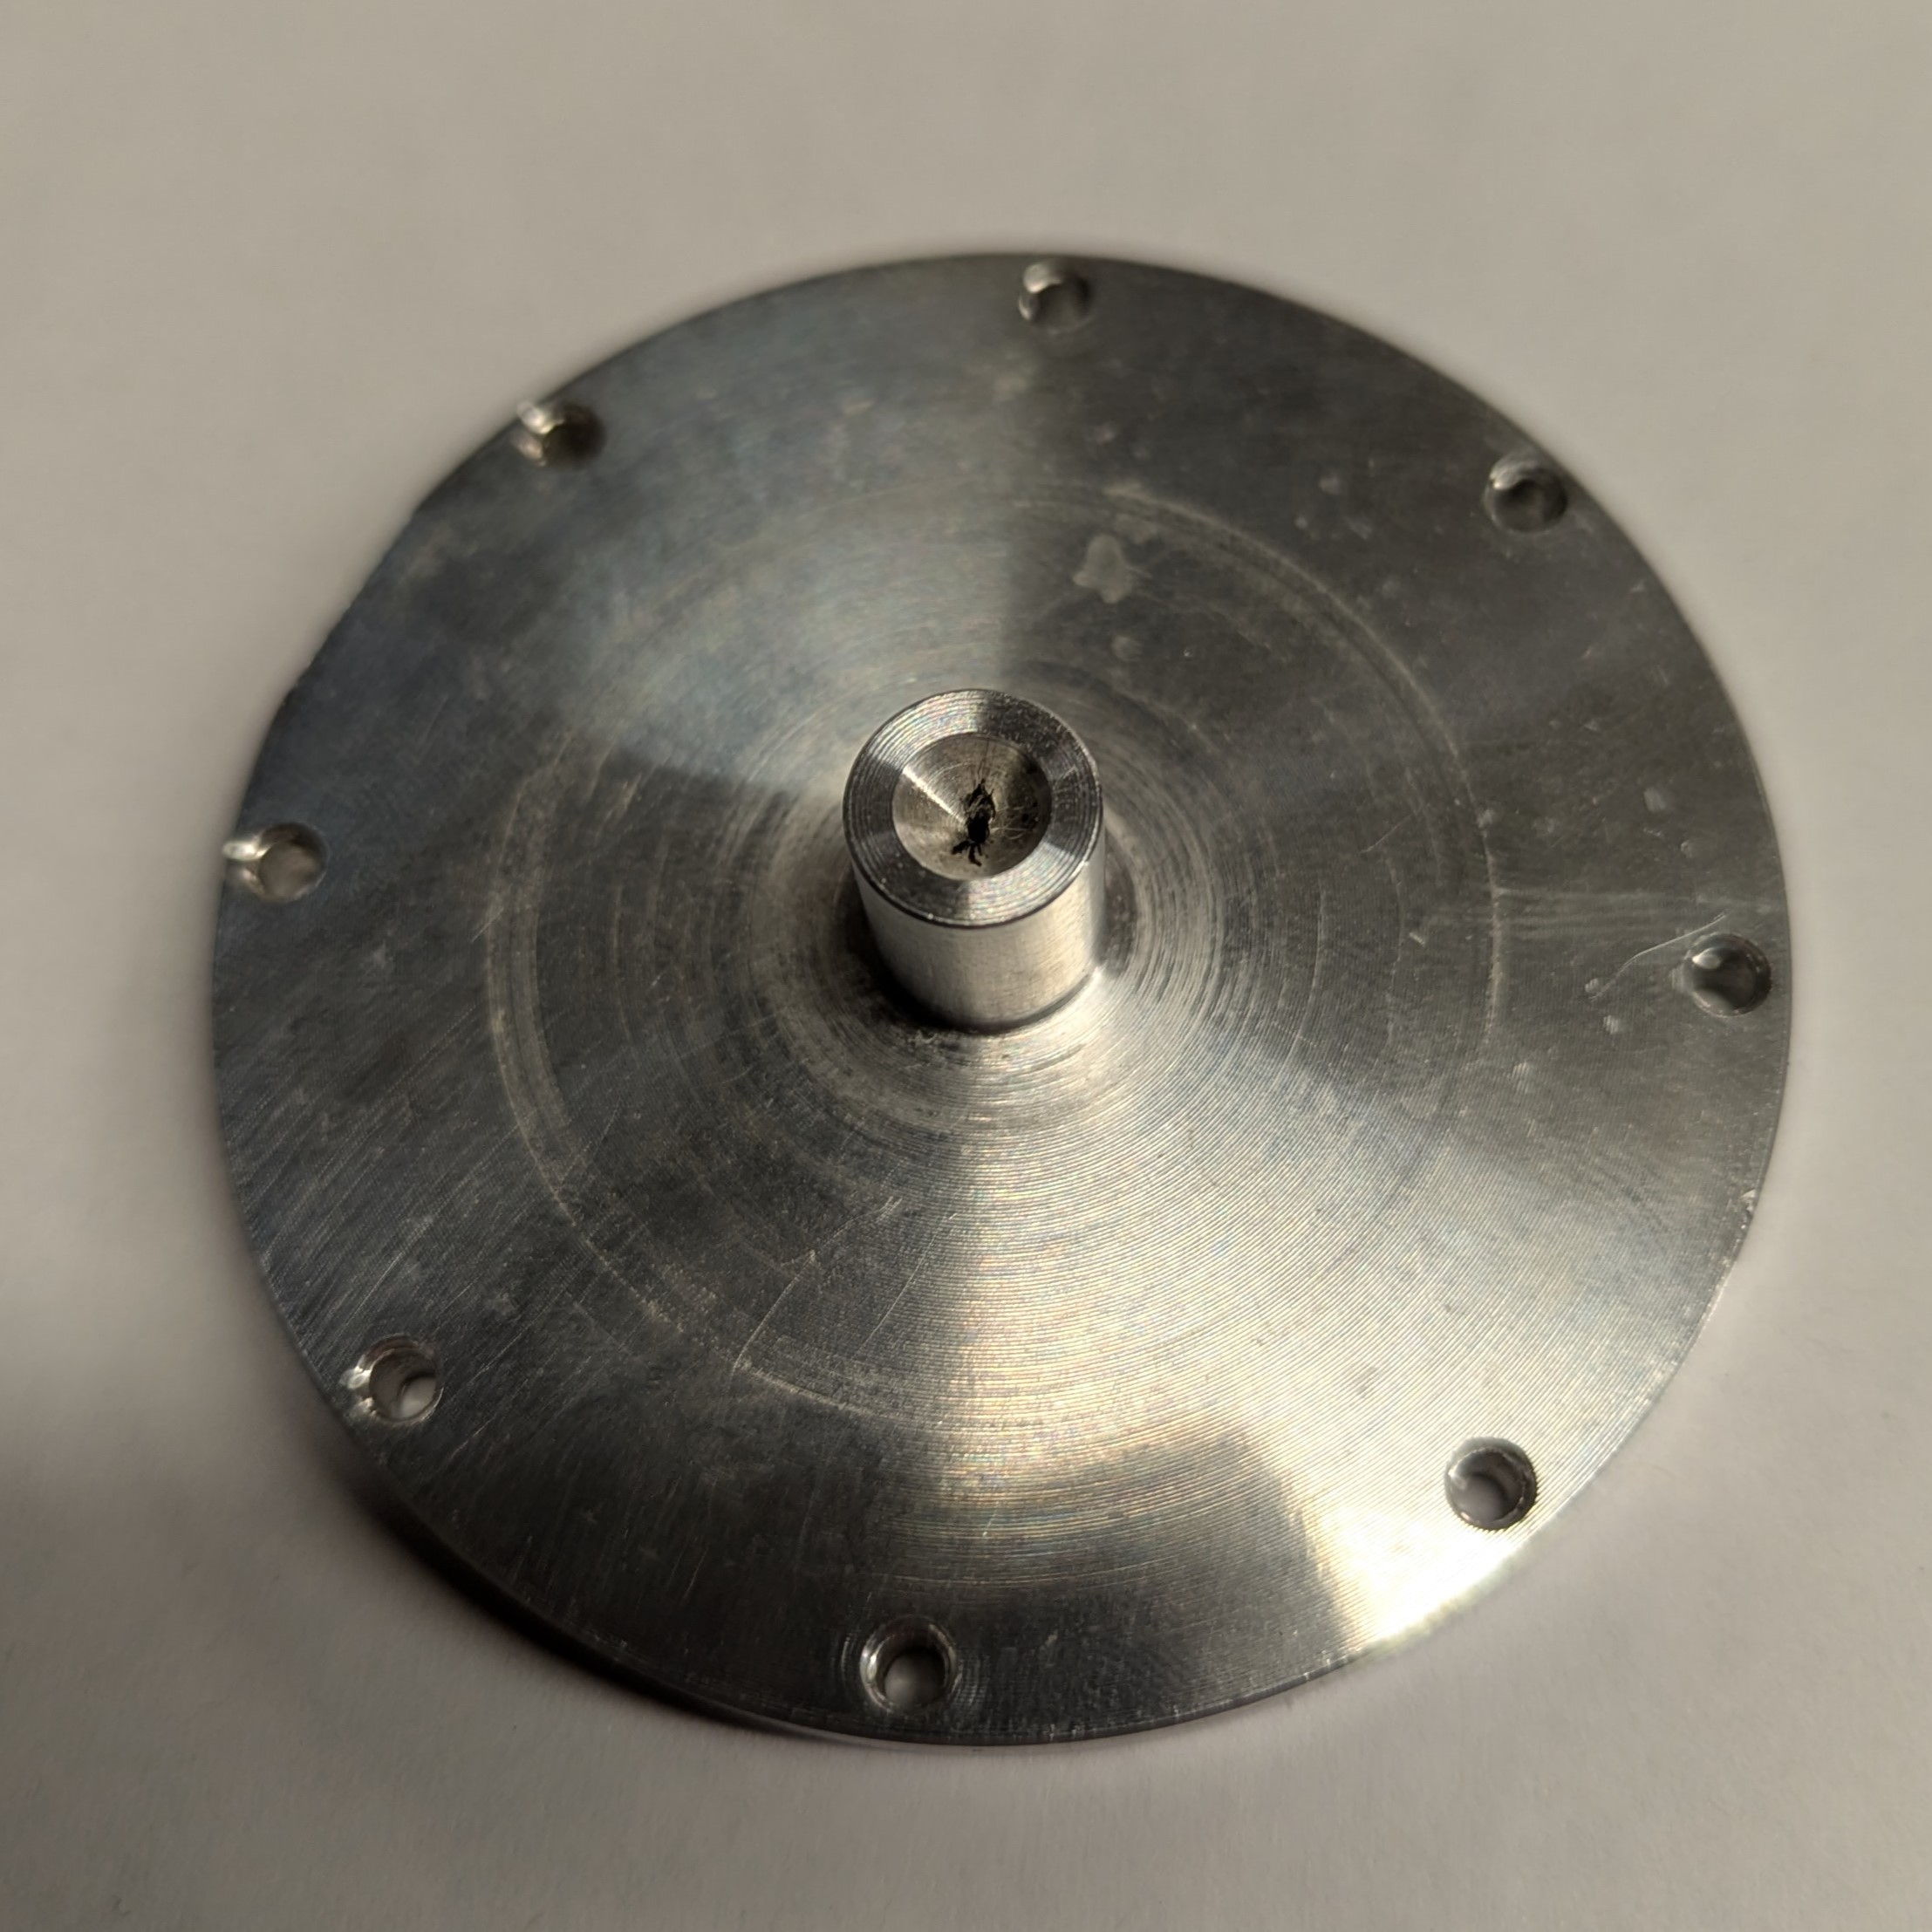
\includegraphics[width=0.45\textwidth]{assets/4 experiments/Nozzle damage.jpg}
    \caption{Nozzle laser damage}
    \label{fig:Nozzle laser damage}
\end{figure}

To solve the ablation of the aluminum nozzle under pulsed laser shots, a new backplate (\autoref{fig:nozzle plate} and \autoref{chp:Exchangeable nozzle plate}) was manufactured to accept nozzle inserts. \textcite{toyodaThrustPerformanceCW2002} use a refractory metal, tungsten, as the nozzle material. Other possibilities are machinable ceramics, stainless steel or graphite. Graphite was chosen as it was already used by \textcite{shojiLaserheatedRocketThruster1977} and was economical. These inexpensive, changeable inserts (\autoref{fig:nozzle insert} and \autoref{chp:New nozzle}) were made from superfine iso-molded graphite rods sourced from Graphitestore (0.500" diameter x 12"L, SKU GT001685). V2's inner cylinder was also re-machined (\autoref{chp:remachined inner cylinder}) to guarantee a seal with the new nozzle. Due to machining delays, these final parts are still to be tested.

\begin{figure}[!ht]
    \centering
    \begin{subfigure}[t]{0.45\textwidth}
        \centering
        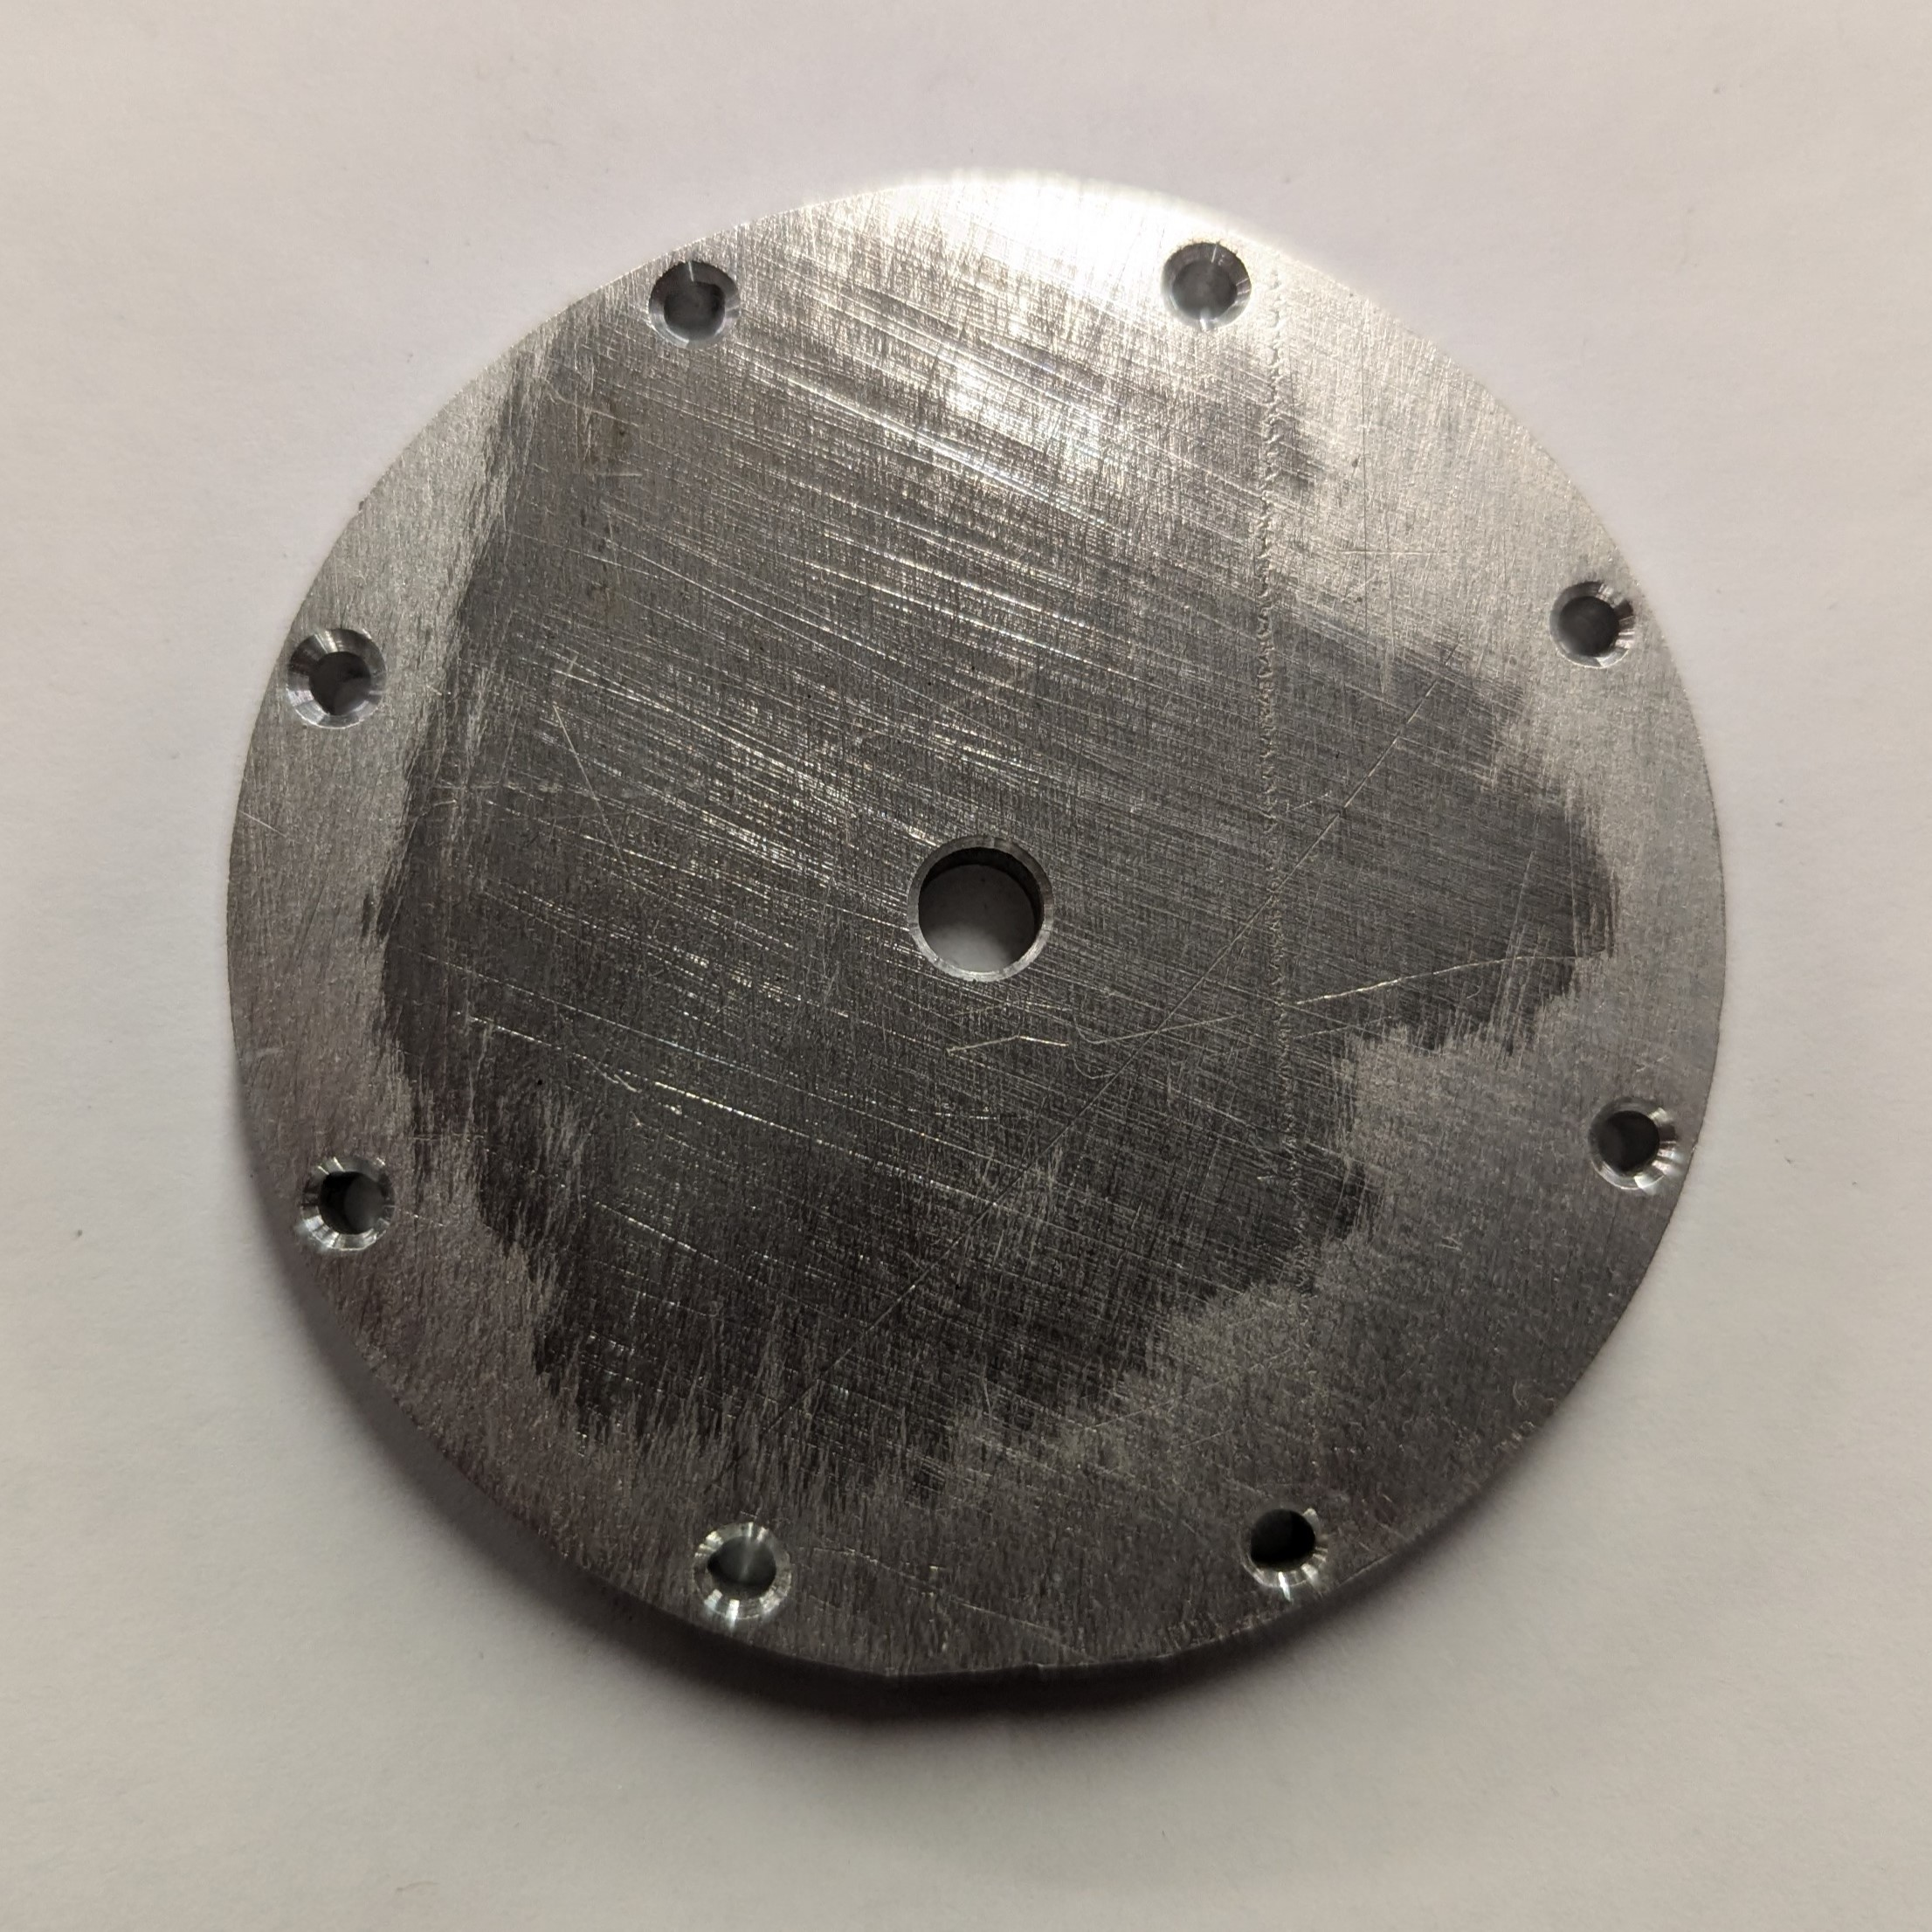
\includegraphics[width=\textwidth]{assets/5 discussion/Nozzle plate.jpg}
        \caption{Nozzle retention plate}
        \label{fig:nozzle plate}
    \end{subfigure}
    \hfill
    \begin{subfigure}[t]{0.45\textwidth}
        \centering
        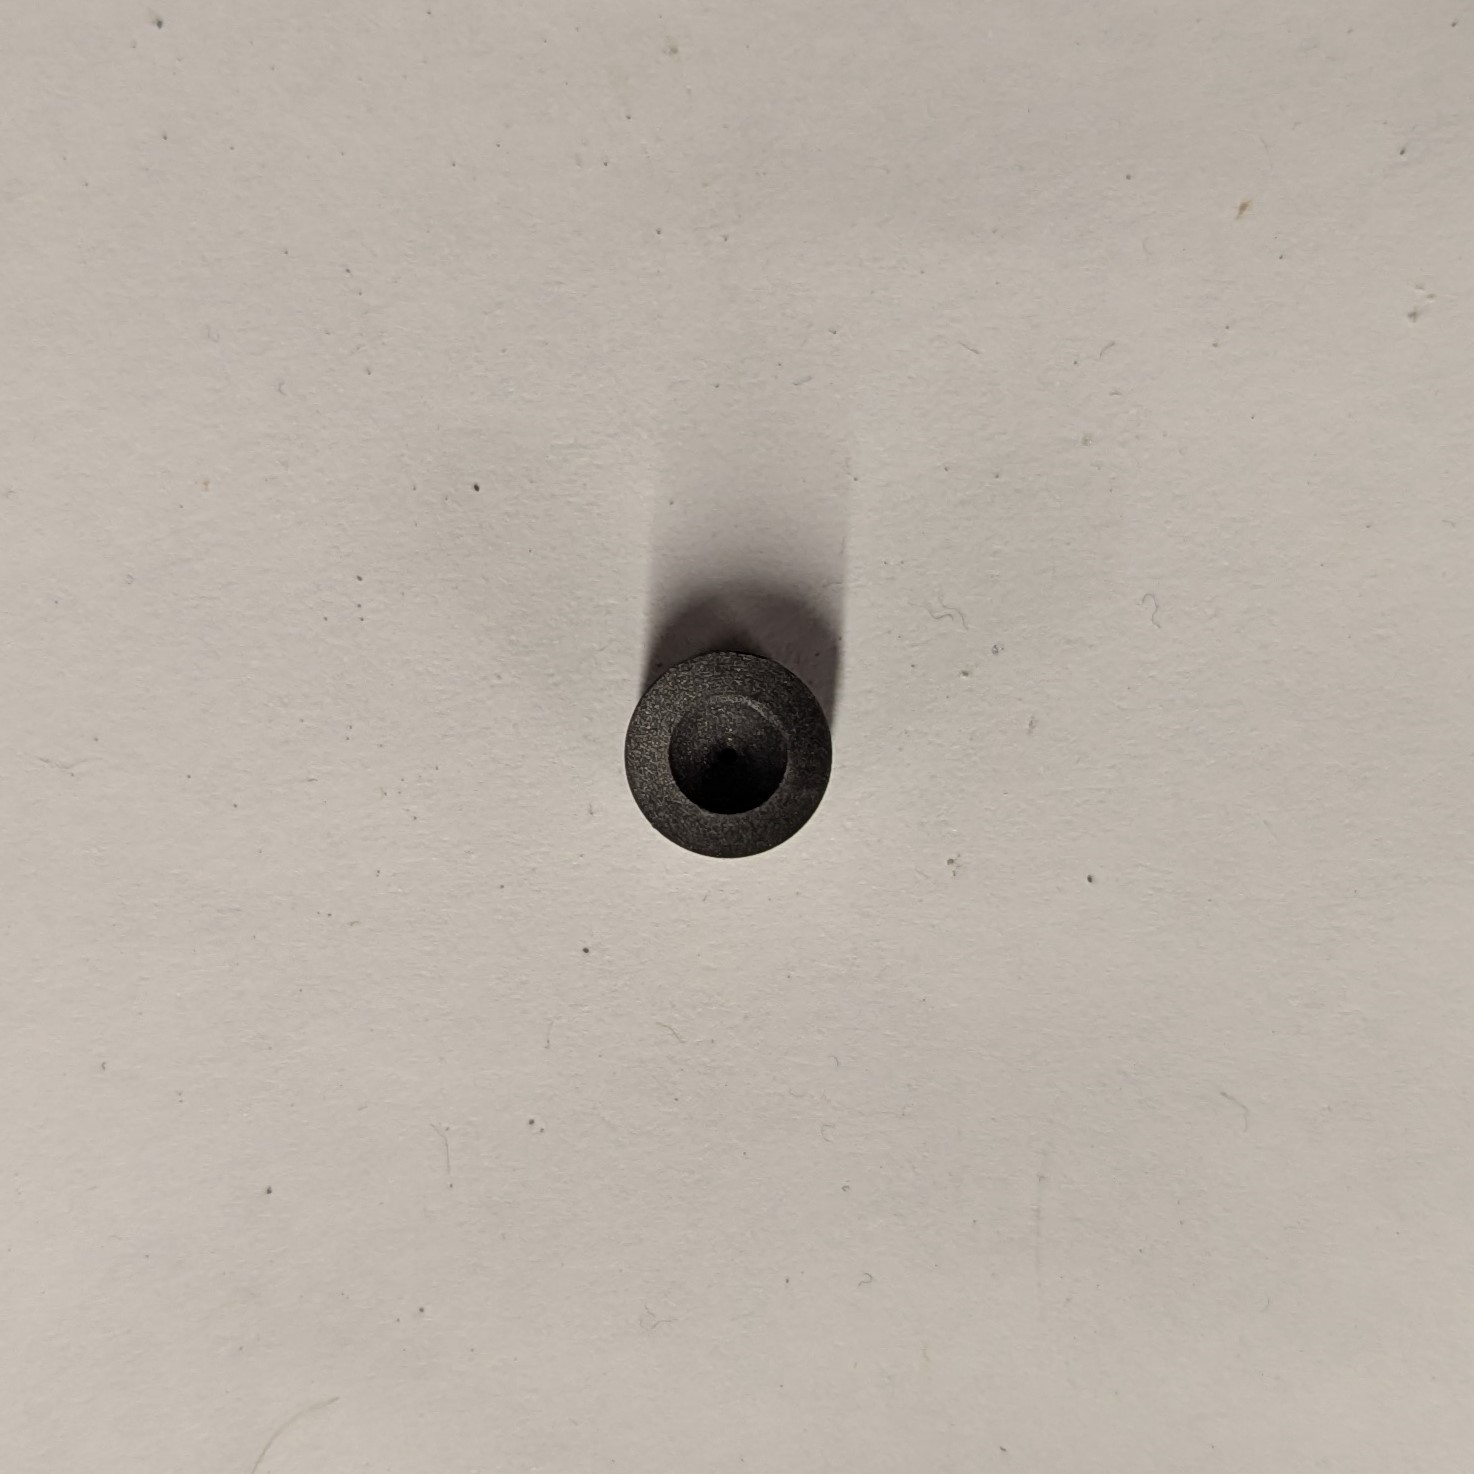
\includegraphics[width=\textwidth]{assets/5 discussion/Nozzle insert.jpg}
        \caption{Graphite nozzle insert}
        \label{fig:nozzle insert}
    \end{subfigure}
    \caption{New nozzle parts}
\end{figure}

Longer term, to ultimately test LTP as a viable means of space propulsion, more improvements to the V2 setup can be envisioned. A simple but costly one is to use a more powerful laser, instead of the \qty{300}{W} CW one used here. This would increase thrust and laser absorption by the plasma, making an eventual thrust increase easier to detect. Using hydrogen as a propellant instead of argon would increase the thruster's specific impulse. However, it would be harder to ionize, possibly requiring higher laser power or better focusing optics. A hydrogen LTP thruster would also need to be run inside a vacuum chamber, as hydrogen is extremely flammable.

\section{Model discussion}

    Using a model for Bremsstrahlung loss, the zero-dimensional (0D) heat transfer model successfully approximated the order of magnitude and the timescale of the first of two pressure increases seen in experiments (\autoref{fig:LSP178_SPRK49}). The second, higher, peak could be explained by the fact that after the laser pulse, the energy in the cone was then communicated to the bulk argon volume. This equalization of temperatures and pressures could be due to natural convection. To test this hypothesis in future studies, the timescales of radiation and convection should be determined with the geometry of the problem.

    In \autoref{fig:Two further LSPs}, the model increasingly overshot the experimental pressure data as the laser power was decreased. A potential cause for this was that laser energy transmission was not taken into account in the model, and a measurement of this transmission was not taken experimentally. As the laser power was lowered, the fraction of laser energy that was absorbed by the plasma (laser absorption efficiency) also decreased.
    
    The LSP growth mechanism (\autoref{fig:Mechanism of LSP growth}) was also not modelled, but it is useful to understand the physics at play.

    \begin{figure}[!ht]
        \centering
        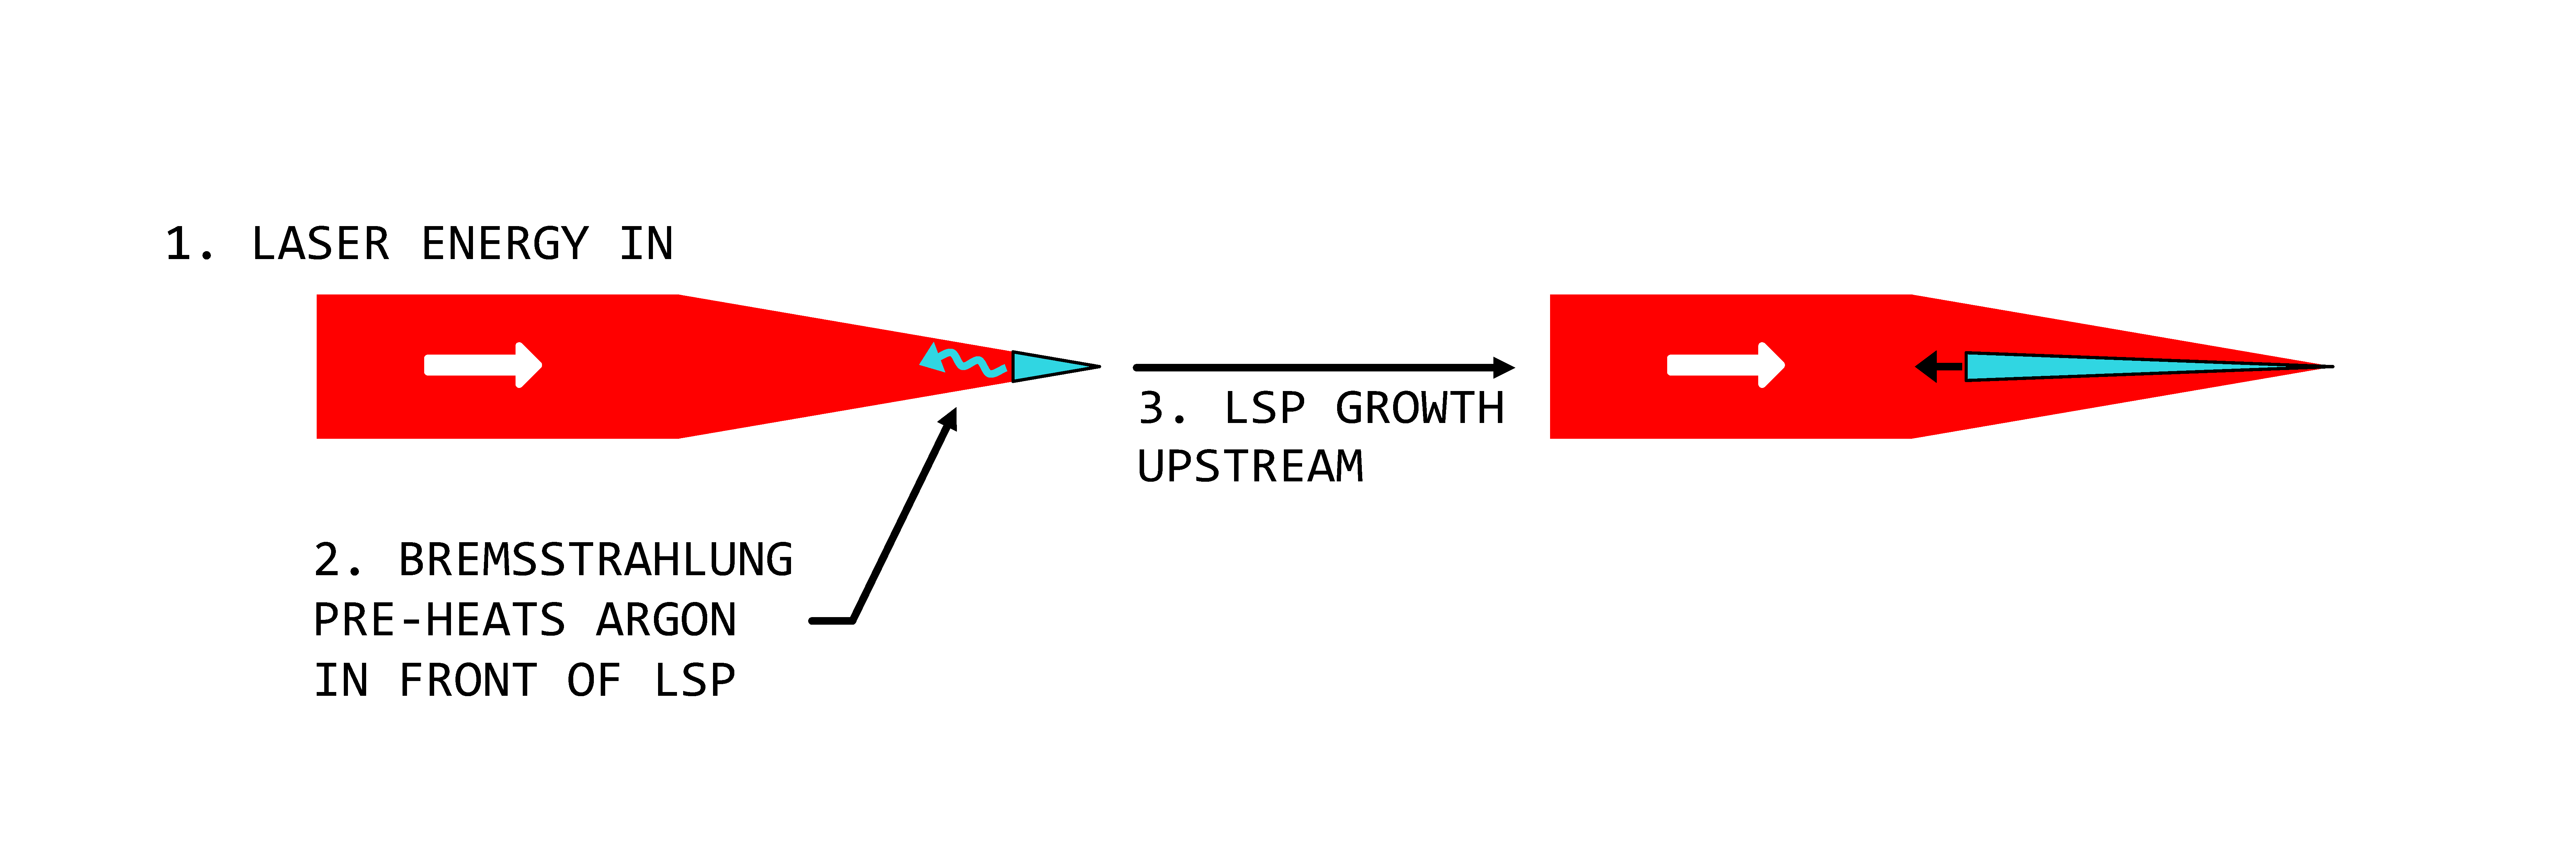
\includegraphics[width=0.85\textwidth]{assets/2 models/Mechanism of LSP growth.pdf}
        \caption{Mechanism of LSP growth}
        \label{fig:Mechanism of LSP growth}
    \end{figure}

    The laser creates at first a small LSP volume near the focus, where the laser flux is highest. As the plasma radiates via Bremsstrahlung, the argon around the plasma is heated. Being exposed to the laser beam, the argon in front of the LSP ionizes. This causes the plasma to propagate towards the laser collimator until equilibrium is reached between radiation and heat dissipation. This reduces the absorption efficiency of the plasma, as the thicker part of the cone is no longer at the laser's focus, where the highest laser flux, and therefore temperature, can be reached. Gas flow up to a certain velocity can be used to push the plasma back into the focus, as was explained in \textcite{chenEmissionSpectroscopyCw1989a}. Too high a gas flow speed, and the plasma is blown out. Future experimental investigation of the V2 thruster could determine what the ideal flow speed is.

% New parts that were made and why?
    % Nozzle/retaining plate
    % Window extension
    %  NPT fitting to calculate m_dot in bubble meter
% ADD IMPORTANT: Due to machining delays however, these final parts were not tested.

% Future work:
% - Validate that window extension works
% - Characterize nozzle throat effective diameter

    